\chapter{绪论}

\section{研究背景与意义}
近年来,我国高度重视人工智能与智能感知技术的发展,将其作为推动经济社会高质量发展的重要引擎。
2025年,国务院印发《关于深入实施“人工智能+”行动的意见》,明确提出要加快人工智能与实体经济、社会治理和公共服务的深度融合,
重点推进智能感知、智能决策与智能控制等关键技术在交通运输、公共安全、智慧城市、无人系统等典型场景中的规模化应用\cite{AI_Plus_Action_2025}。
在此国家战略背景下,如何提升人工智能系统在真实复杂环境中的感知能力与运行可靠性,已成为当前学术界和产业界共同关注的核心问题。

多目标检测与跟踪作为计算机视觉与智能感知领域的重要研究方向,是实现环境理解、行为分析和智能决策的基础技术之一。
该技术通过对视频序列中多个目标进行持续识别、定位与身份保持,为上层决策系统提供结构化的时空信息支撑,已在多个实际场景中得到广泛应用。
\autoref{fig:ch1_1}给出了多目标检测与跟踪技术在典型应用场景中的实例,包括智能交通、自动驾驶、体育赛事分析以及无人系统等方向。
% 随着智慧交通、低空经济和无人系统的快速发展,这些应用场景对多目标检测与跟踪算法在复杂环境下的稳定性、鲁棒性与泛化能力提出了更高要求,其性能直接关系到智能系统在真实场景中的运行安全与决策可靠性。

\begin{figure}[htbp]
    \centering
    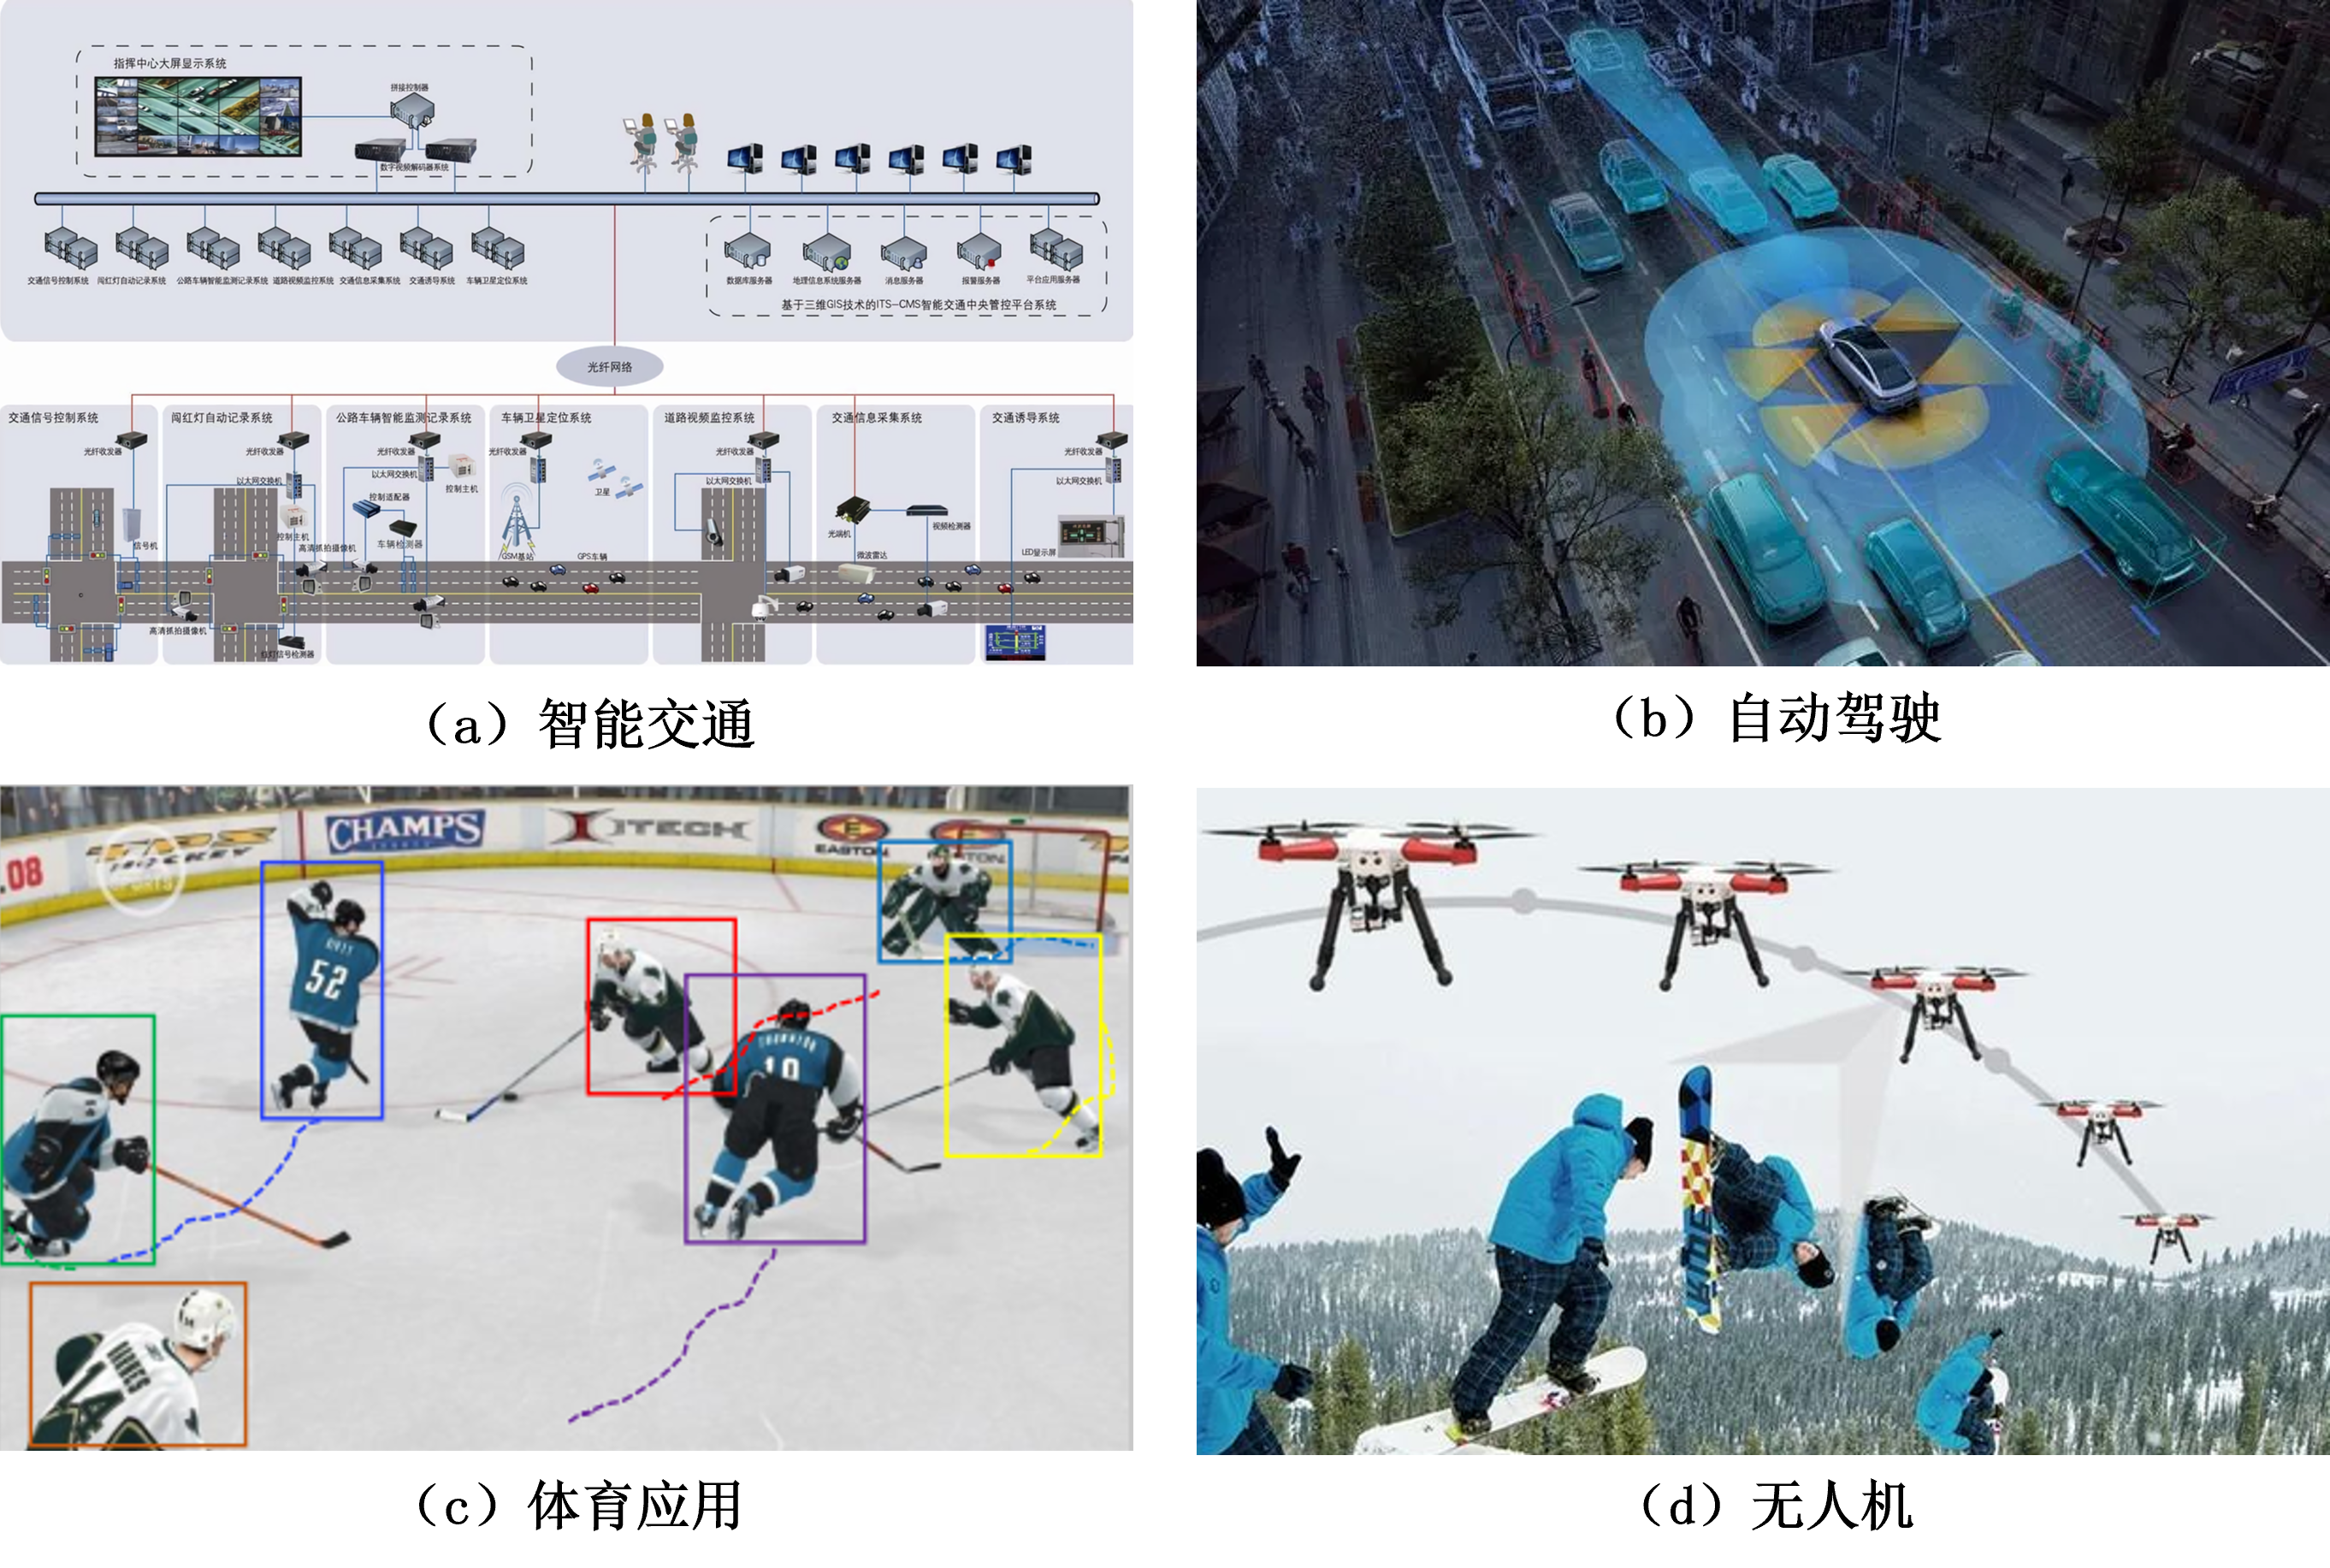
\includegraphics[width=14cm]{chapter1/1.png}
    \caption{\label{fig:ch1_1}多目标跟踪应用实例}
\end{figure}

    \textbf{1. 智能交通}。根据交通运输部的统计数据,2024年我国完成城市客运量达到1067.97亿人次,较2023年增长5.7\%\cite{MOT_2024_Stats}。
面对如此庞大的人流与车流规模,传统依赖人工或规则的交通管理方式已难以满足高效、精细化管理需求。
基于多目标检测与跟踪技术的智能交通系统通过对道路交通参与者进行实时感知与持续跟踪,可为交通流量分析、拥堵预警和交通信号控制优化提供关键数据支撑,
已成为了现代交通管理的重要技术手段。如百度公司与中山大学合作开发了一种在线运动车辆技术系统\cite{Lu2021VehicleCounting},该系统旨在对交通复杂、拥堵的十字路口进行车流量分析。
通过实时监控和数据分析,该系统能够提供准确的车流信息,有助于交通管理部门在高峰期进行科学的交通调控,缓解路口拥堵,提升整体交通流效率。
同时,这一系统的引入也有助于提高路口的车辆通行能力和信号灯的工作效率,为进一步优化城市交通管理提供了技术支持。

    \textbf{2. 自动驾驶}。车辆需要在动态、复杂且高度不确定的交通环境中实现安全行驶,这对环境感知系统提出了极高要求。
多目标跟踪技术通过持续感知并预测周围行人、车辆等多类目标的运动状态,为自动驾驶系统的路径规划和决策控制提供基础信息,是实现高等级自动驾驶不可或缺的关键技术之一。
如广汽研究院X lab团队提出了一种创新的多目标跟踪算法,在自动驾驶行业内首次将跟踪的多视角数据通过深度学习方法转换到鸟瞰图特征空间下,并在国际权威的自动驾驶测试竞赛中获得纯视觉榜单全球第一。

    \textbf{3. 体育应用}。体育赛事因其精彩纷呈而广受大众喜爱,一般观众通常关注精彩瞬间或喜爱的运动员,而专业球迷、运动员、教练以及媒体从业者则更倾向于比赛的深入分析。
为满足这些不同需求,多目标跟踪技术在体育比赛分析中发挥了重要作用。通过对球员和球体的精准跟踪,该技术为运动员表现评估、战术调整、团队合作优化以及比赛再编辑提供了科学依据,
提升了比赛的观赏性和技术分析的精准性。如2022年的北京冬奥会引入的“3D运动员跟踪技术”,该技术基于多目标跟踪算法,能够实时检测并捕捉运动员的速度、加速度、运动方向和运动轨迹等数据,
进而生成运动员的3D形态信息。通过这些数据的分析,该技术能够提取并生成每个运动员的精彩比赛瞬间,并在直播过程中即时回放,为观众带来更加沉浸式的观看体验。

    \textbf{4. 无人机}。随着无人机技术的不断成熟,其在军事和民用领域的价值不断凸显。在军事方面,无人机不仅提升了战场感知能力,其实时性强、隐蔽性好、抗干扰能力佳的特点,使它能够快速、准确地收集情报,
同时避免人员直接暴露于危险之中;在影视制作和体育赛事中,无人机能够自动跟随拍摄对象,提供稳定、流畅的空中拍摄画面;在搜索救援中,无人机可以自动跟随搜救人员,提供空中视角,
帮助搜救人员更高效地开展救援工作。目前,目标跟踪技术已在商业领域实现实际应用,并具备实时对拍摄对象进行自动对焦的能力。以大疆创新公司为例,其开发的无人机产品如Mini 3、Air 3等,
均配备了先进的智能跟随系统,允许无人机能够在无需人工干预的情况下自动跟随特定目标。

尽管多目标跟踪技术在智能交通、视频监控与自动驾驶等应用场景中展现出巨大的应用潜力,
但在实际部署过程中仍面临诸多关键挑战。
如\autoref{fig:mot_challenge_examples}所示,复杂真实环境下的多目标跟踪任务通常伴随着多种不利因素的共同作用,
包括目标之间频繁的遮挡与交互、外观特征随光照和视角变化而显著波动、检测结果的不稳定性以及相机自身的运动等。
在实际场景中,这些问题往往并非孤立出现,而是相互叠加,
使得目标的外观表征与运动模式呈现出较强的不确定性,
进而引发目标身份频繁切换、轨迹中断等问题,严重影响系统的稳定性与可靠性。
因此,如何在复杂多变的环境条件下综合考虑检测不确定性与目标间的时空关系建模,实现鲁棒、高效的多目标跟踪算法, 已成为当前亟待解决的关键科学与工程问题。
\begin{figure}[htbp]
    \centering
    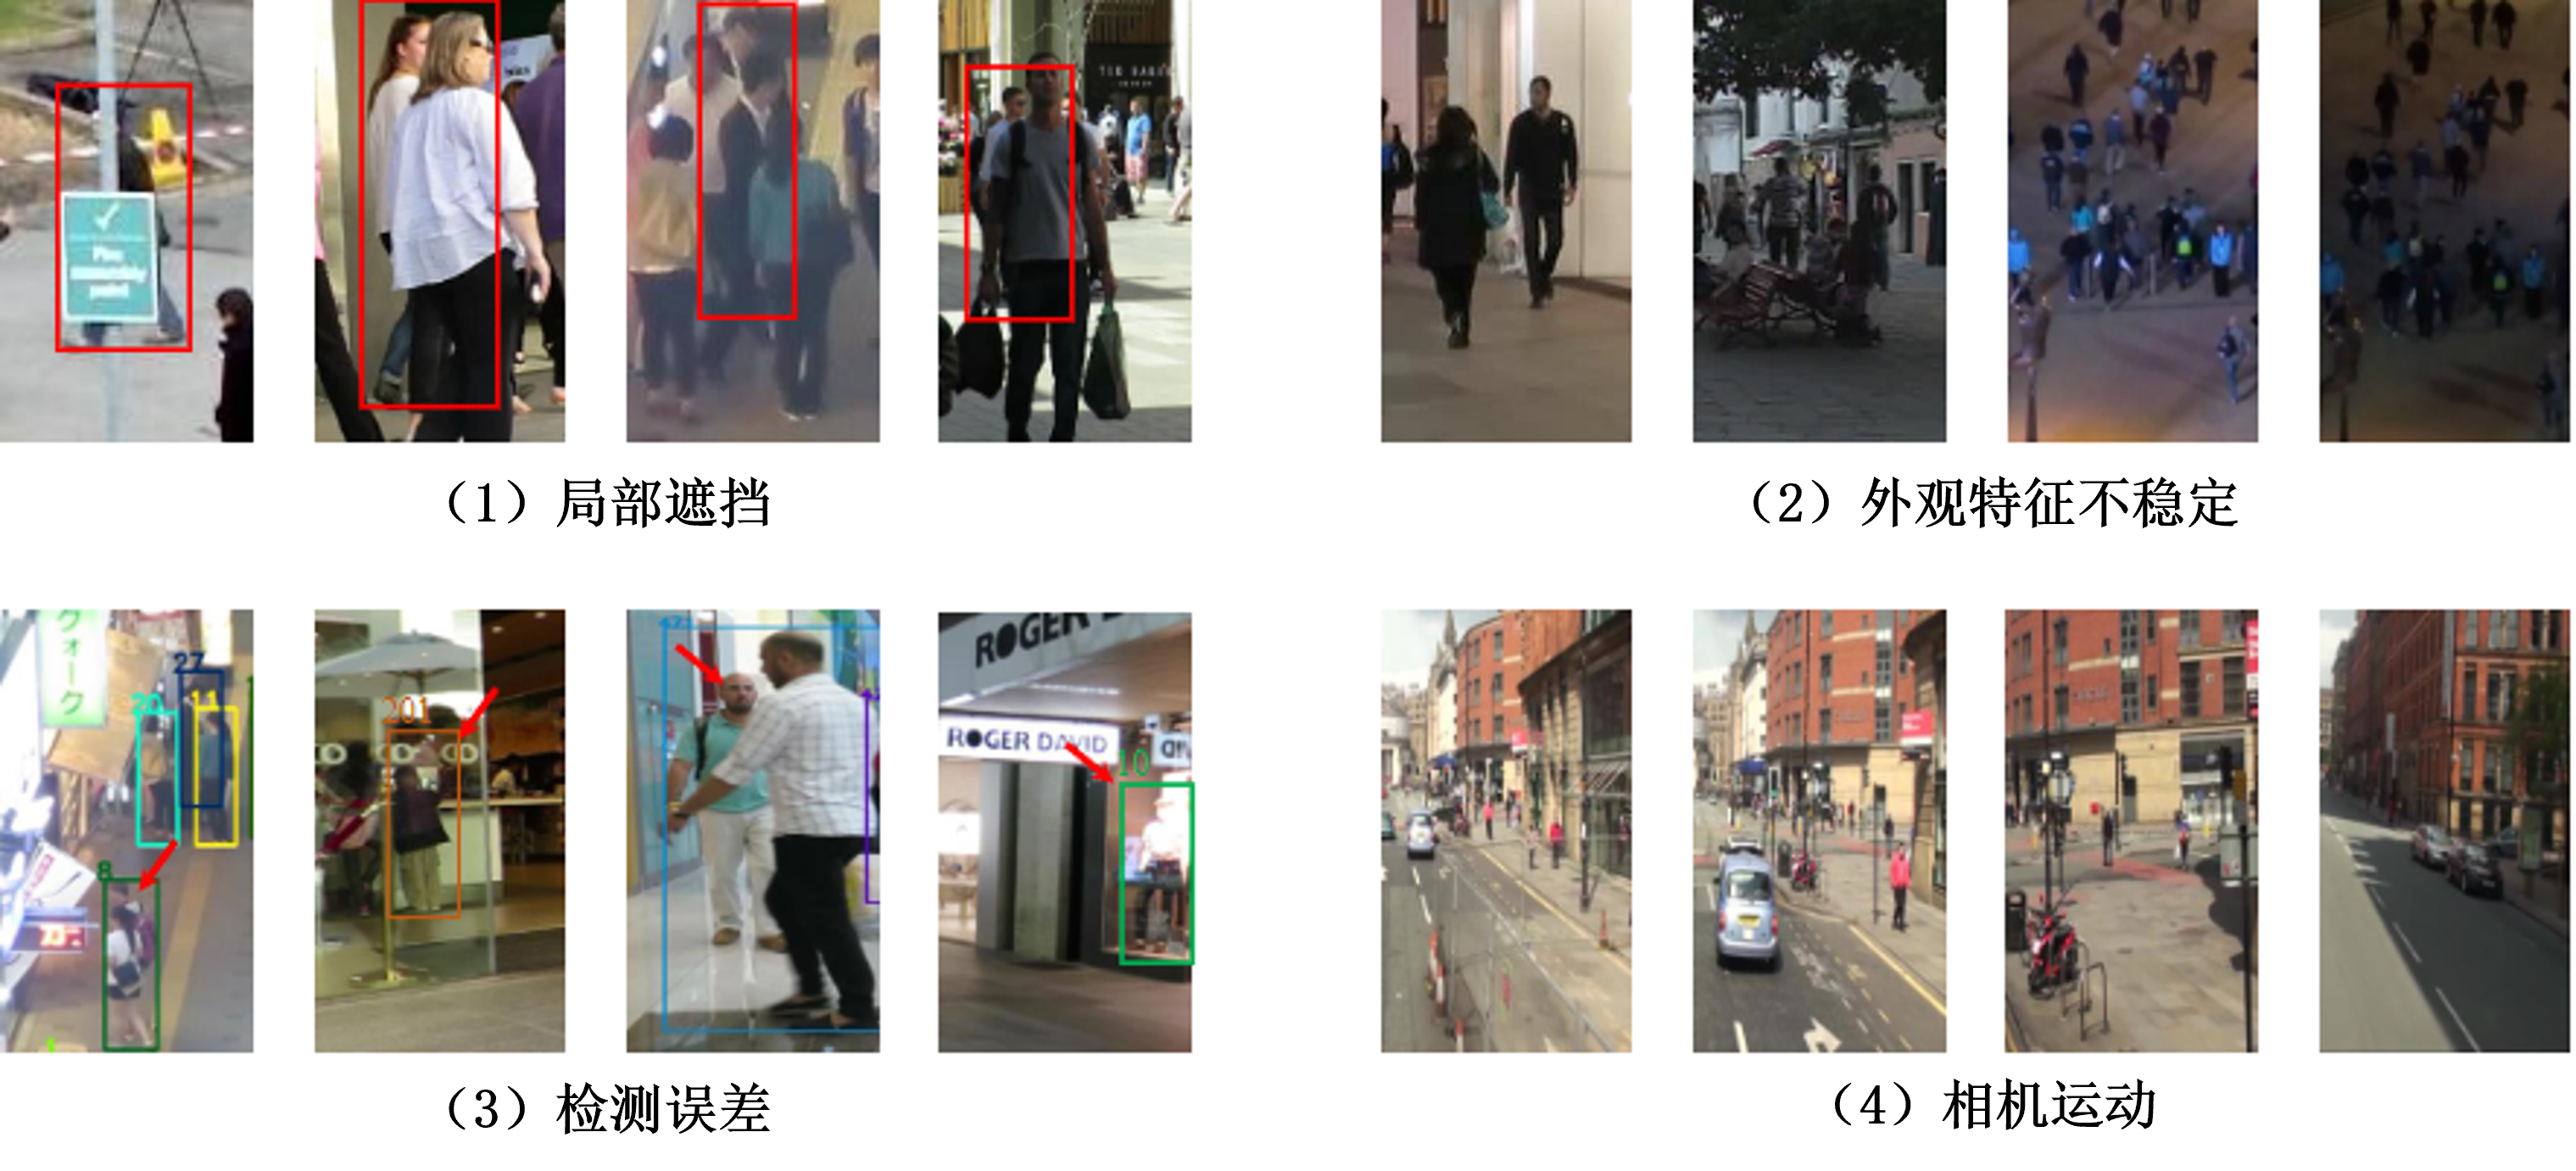
\includegraphics[width=15cm]{chapter1/22.png}
    \caption{\label{fig:mot_challenge_examples}复杂环境下多目标跟踪面临的典型挑战示例}
\end{figure}

\section{国内外研究现状}
\subsection{基于深度学习的多目标跟踪算法概述}

多目标跟踪(Multiple Object Tracking,MOT)任务需要对视频序列中多个目标(一般为行人、车辆或者动物等)的位置和大小进行估计,然后给他们分配一个一般由数字表示的独特标识。
并保持这样的身份标识在所有视频帧中的一致性,最终生成每个目标的运动轨迹。
目前主流多目标跟踪算法遵循基于检测的跟踪(Tracking By Detection,TBD)范式,即将该任务分为目标检测(Object Detection)和轨迹关联两部分。
本节主要从以下两方面对多目标跟踪的研究现状进行简单回顾:多目标跟踪中的目标检测和多目标跟踪中的轨迹关联。

\begin{figure}[htbp]
    \centering
    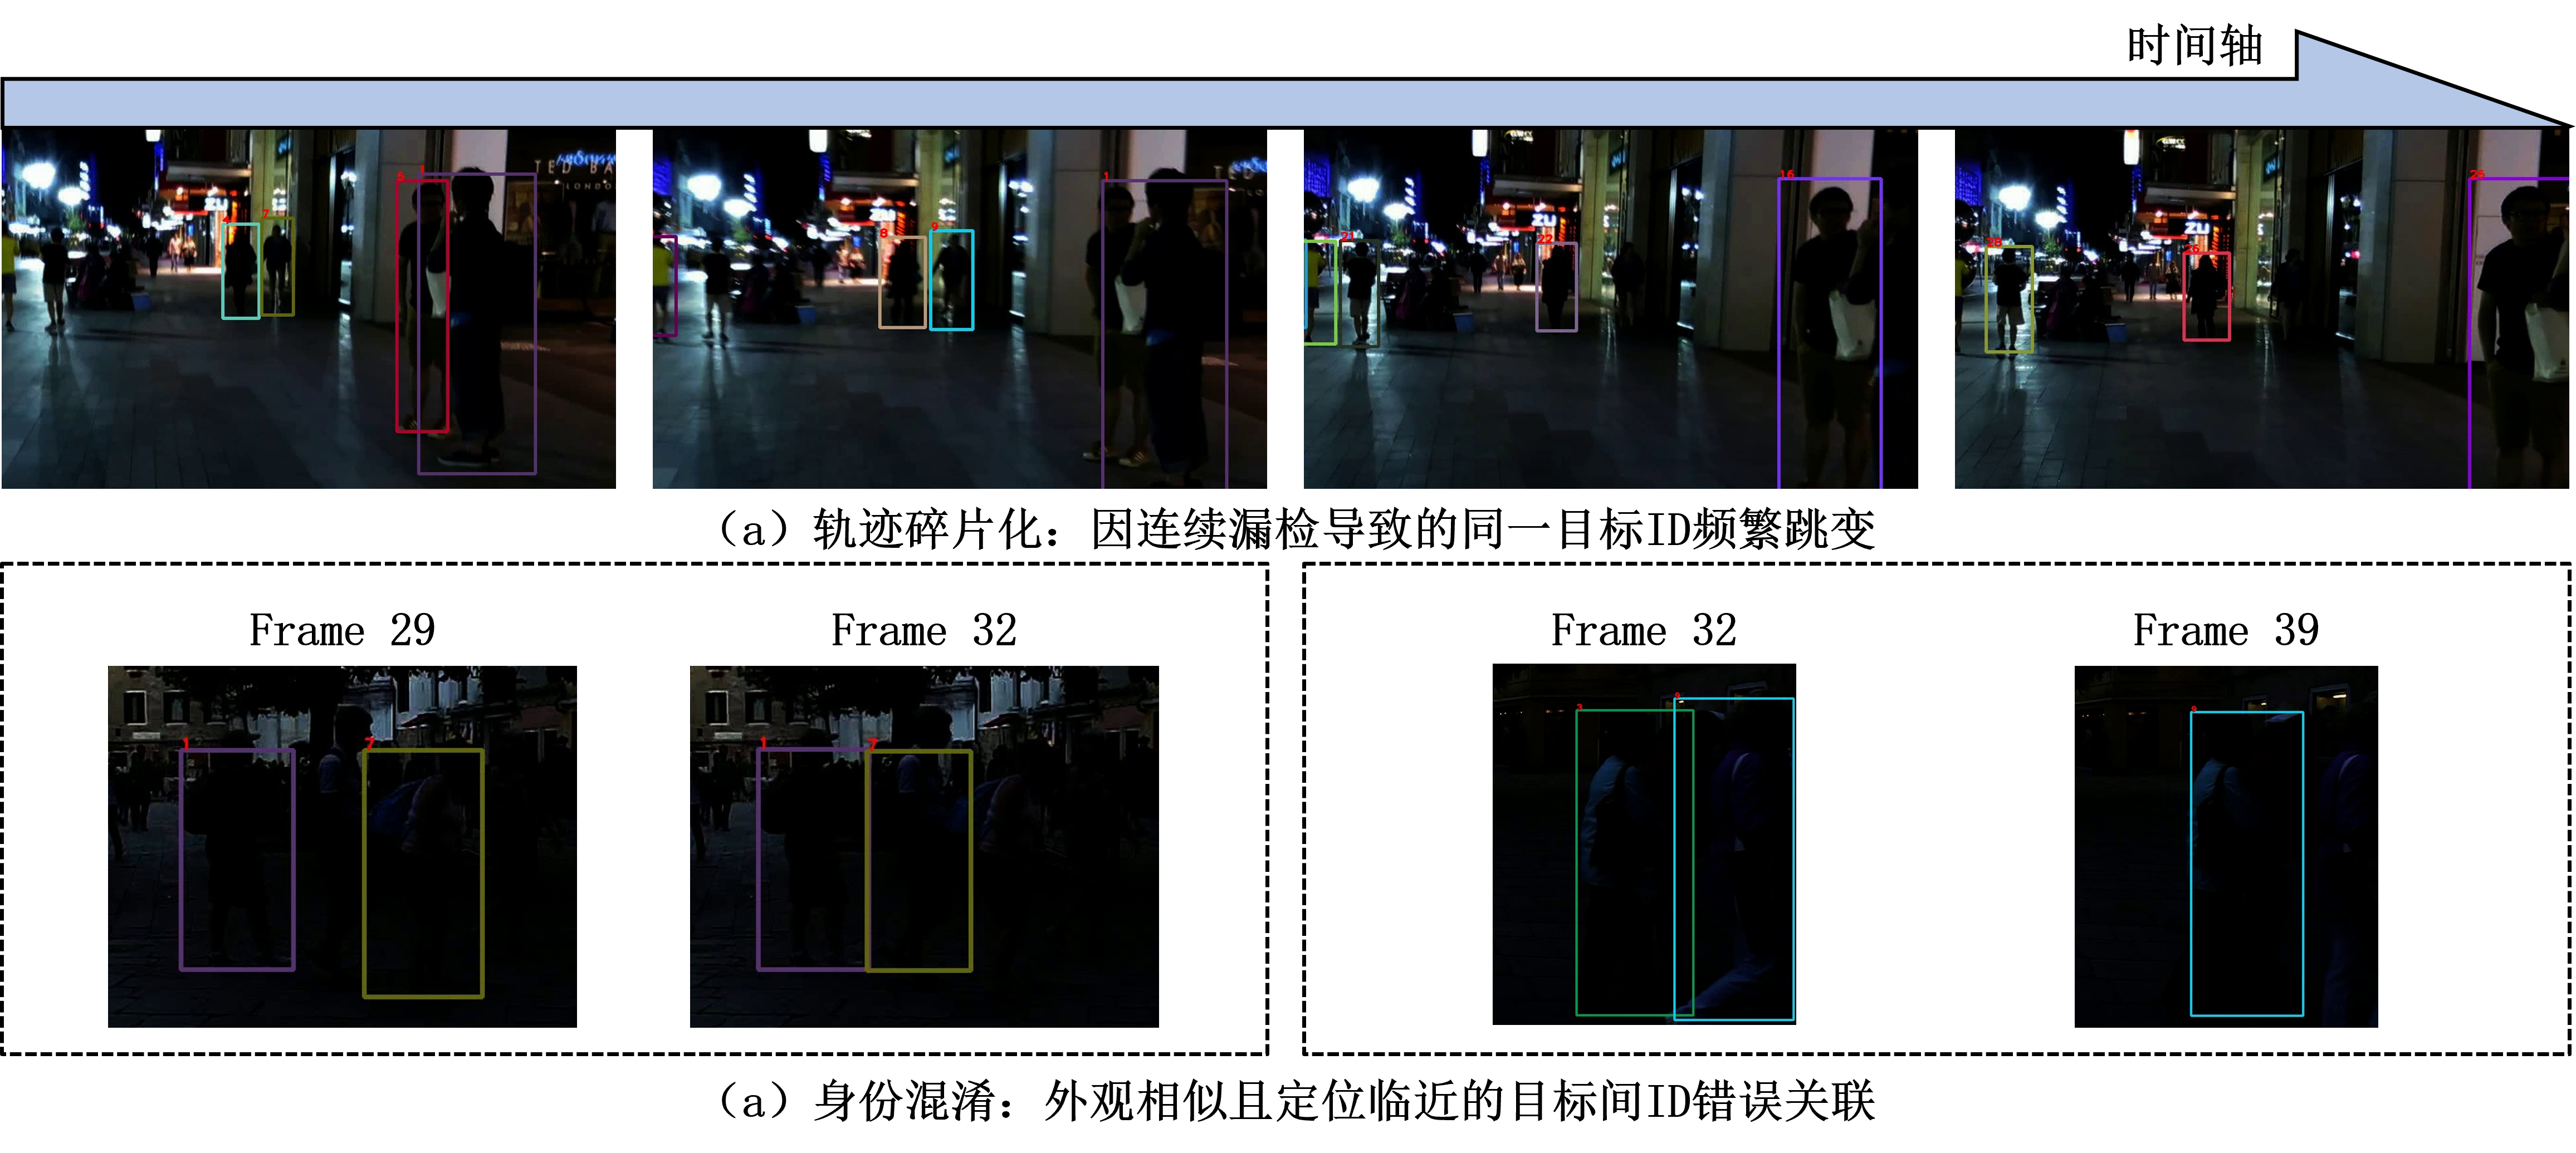
\includegraphics[width=16cm]{chapter1/2.png}
    \caption{\label{fig:ch1_2}基于检测的跟踪范式流程图}
\end{figure}

\textbf{1. 多目标跟踪中的目标检测}
% \subsubsection{多目标跟踪中的目标检测}

现有的多目标跟踪算法中,基本都是基于检测实现的。常用的检测器从不同的角度出发可以分为不同的类别。
从网络层级来看,可以分为双阶段检测器(如Faster RCNN\cite{FasterRCNN},Mask RCNN\cite{maskrcnn})和单阶段检测器(如SSD\cite{ssd},YOLO\cite{yolov1});
从是否使用预定义的锚框(Anchor Boxes)来预测目标的位置,可以分为基于锚框的检测器(如Faster RCNN)和无锚框的检测器(如CenterNet\cite{centernet})。

在双阶段检测算法中,以Faster RCNN为例,给定一张图片,首先通过主干网络提取特征图,然后,将这些特征图喂入到候选框提取网络(Region Proposal Network,RPN),来得到一系列可能包含目标的候选框。
每个候选框对应于原图中的一个感兴趣区域(Region of Interest,RoI),再通过感兴趣区域池化(RoIPooling)操作提取对应的特征。
最后,所提取到的特征同时喂入分类子网络和回归自网络,以实现目标识别和细化候选框位置。对于不包含检测目标的检测框,则将其归类为背景类别。Faster RCNN的速度和检测精度方面上均领先于同期其他算法。

\begin{figure}[htbp]
    \centering
    \includegraphics[width=12cm]{chapter1/3.png}
    \caption{\label{fig:ch1_3}Faster RCNN算法流程图}
\end{figure}

在多目标跟踪算法中,SORT\cite{sort}是首次将Faster RCNN作为检测器,进行多目标跟踪的工作。并验证了当检测器性能较好时,仅利用目标边界框的交并比(Intersection over Union,IOU)作为代价函数也能获得较好的跟踪效果。
然而,SORT的检测与跟踪过程是完全独立的,检测部分仅用于为跟踪提供初始位置,后续的跟踪阶段并不与检测过程交互。

与此不同,Tracktor\cite{tracktor}则利用Faster RCNN巧妙地将检测与跟踪过程相结合。具体来说,Tracktor通过将上一帧跟踪到的目标边界框也作为当前帧的候选框,
进行后续的特征提取、分类和回归任务,并保留目标的身份信息,从而无需额外设计跟踪算法简化了流程。

% \begin{figure}[htbp]
%     \centering
%     \includegraphics[width=12cm]{chapter1/4.png}
%     \caption{\label{fig:ch1_4}Tracktor算法流程图}
% \end{figure}
虽然双阶段检测器在多目标跟踪中提升了跟踪精度,
但其高昂的计算成本和较慢的检测速度限制了跟踪效率。为此,一部分研究者转向采用单阶段检测器以加速多目标跟踪过程。

在单阶段检测算法中,与双阶段检测器相比,该类算法摒弃了候选框提取网络RPN,因此在计算复杂度上有所降低,使得检测速度得到显著提升。
此外单阶段检测器在结构上具有更高的灵活性,易于扩展,能够便捷地集成额外的功能分支,如提取目标外观特征的分支等。
下面主要介绍两种在多目标跟踪领域常用的单阶段检测器YOLO和CenterNet。

YOLO算法将检测任务视为回归任务,它直接从图像像素中回归出目标的位置框和类别概率。YOLO首先将输入图像划分为$S \times S$个网格单元,
即生成一个空间尺度为$S \times S$的特征图。然后,将特征图转换为一维向量,并通过全连接层获得最终的输出,直接预测物体的类别和位置框。
最后将输出还原到原始空间尺度,其中每个网格单元包含若干个位置框及其对应的置信度,同时也包含一个目标的类别概率。
由于移除了侯选位置框生成阶段,YOLO可以达到45FPS速度。

\begin{figure}[htbp]
    \centering
    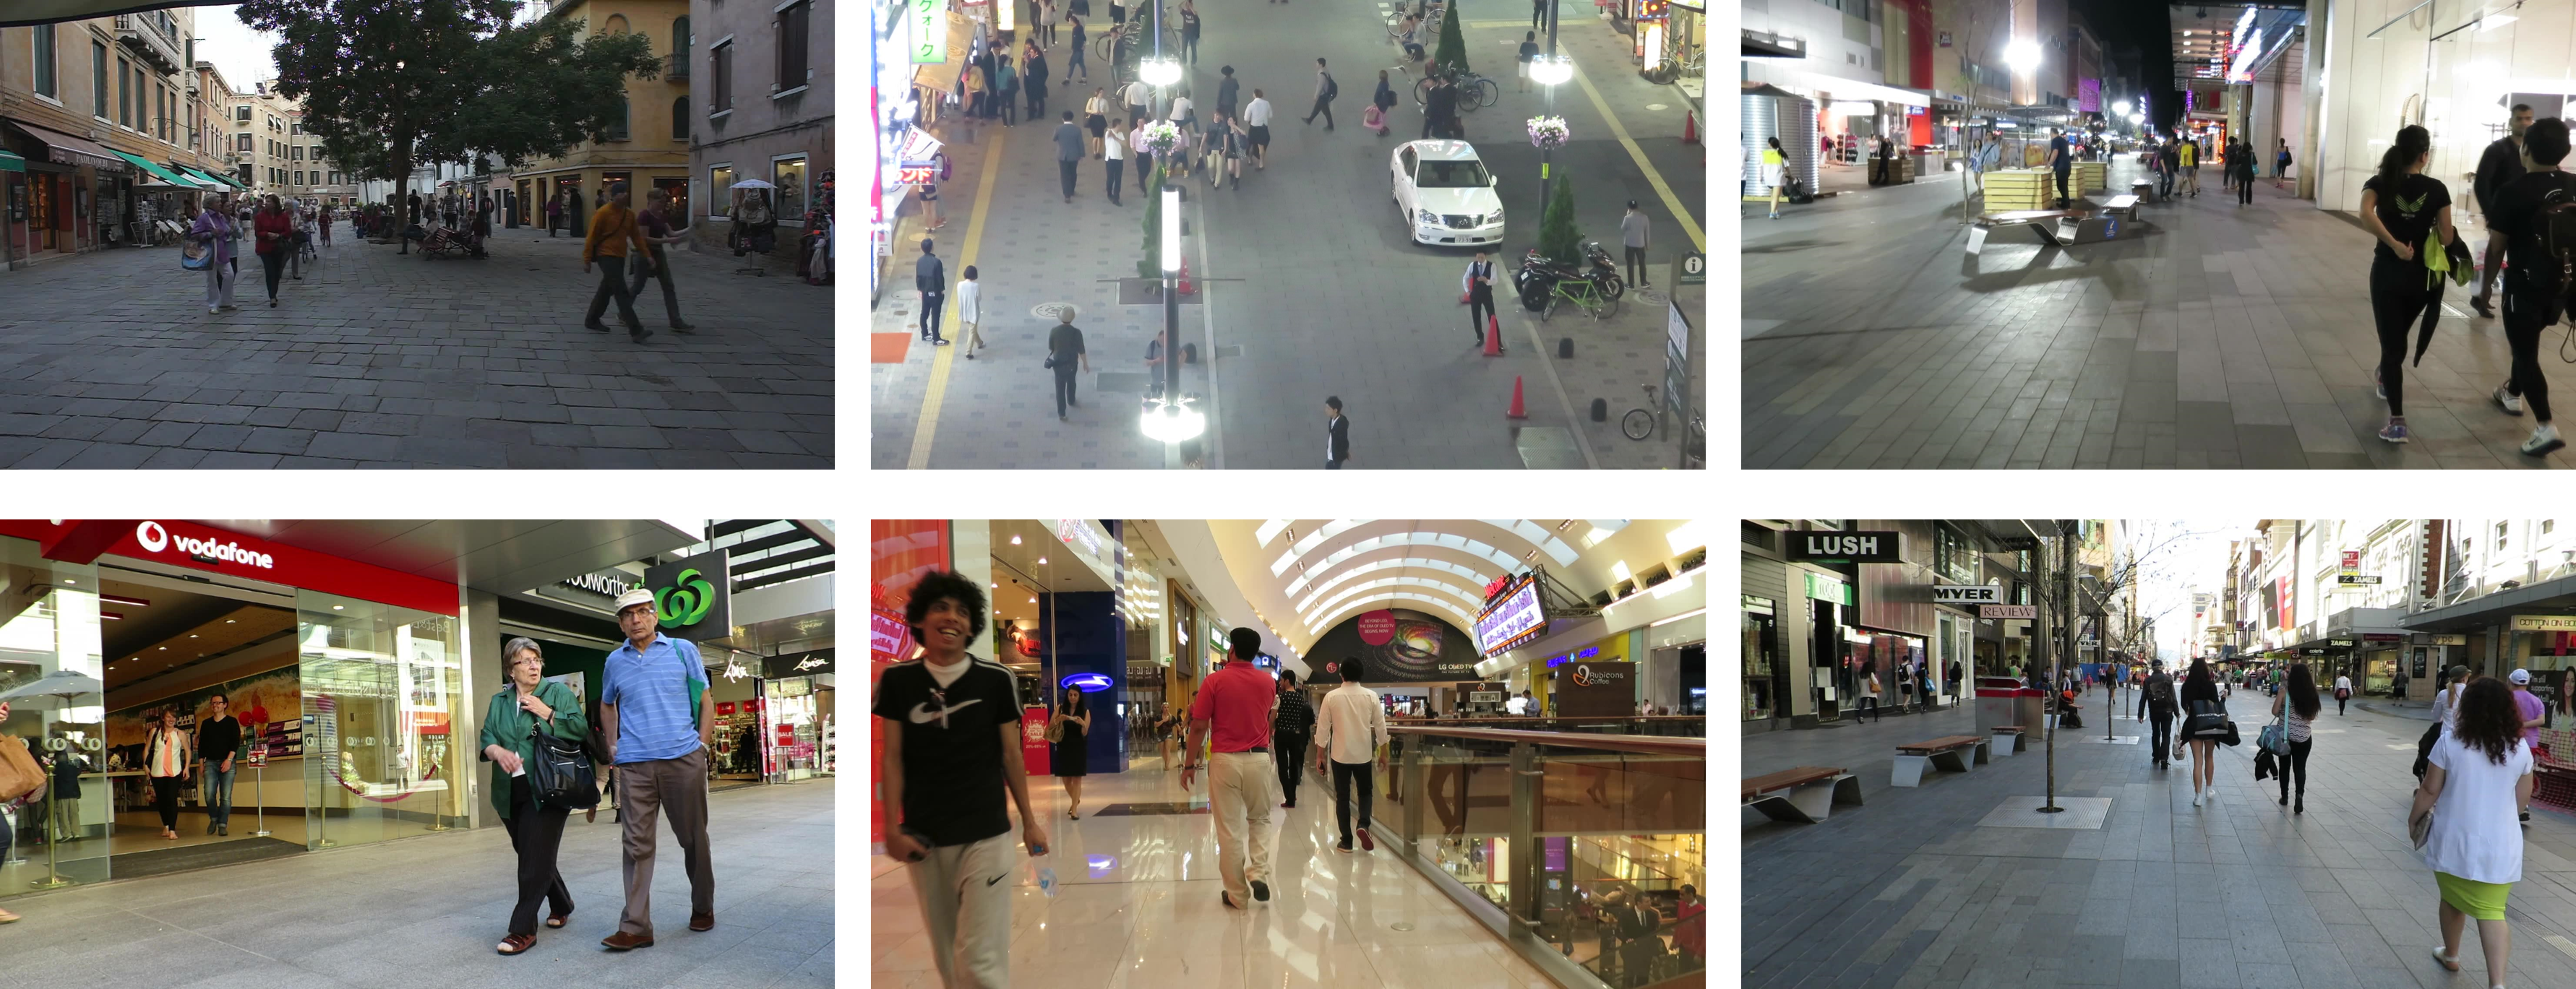
\includegraphics[width=12cm]{chapter1/5.png}
    \caption{\label{fig:ch1_5}YOLO算法流程图}
\end{figure}

CenterNet算法将检测任务视为关键点检测任务。具体而言,给定一张图片,首先通过主干网络提取特征图,并将其分别输入到两个基于卷积层的分支网络。
分支网络中的一个负责检测目标的中心点,输出目标的类别标签和置信度;另一个分支则负责回归目标的尺度信息,即位置框的大小。
每个目标的中心由二维高斯分布表示,其中高斯分布的中心点取值为1,且其方差与目标尺寸成正比。
相比于YOLO,CenterNet具有以下三点优势:

1. 该网络完全基于卷积层构建,能够处理不同尺寸的图像;

2. 将位置框回归和类别标签预测分配到不同分支,便于后续添加其他任务分支且不会影响现有网络;

3. 去除了对位置框的非极大值抑制,取而代之的是对关键点热度图进行局部非极大值抑制,这个过程可以通过卷积操作实现,从而简化了检测流程。

% \begin{figure}[htbp]
%     \centering
%     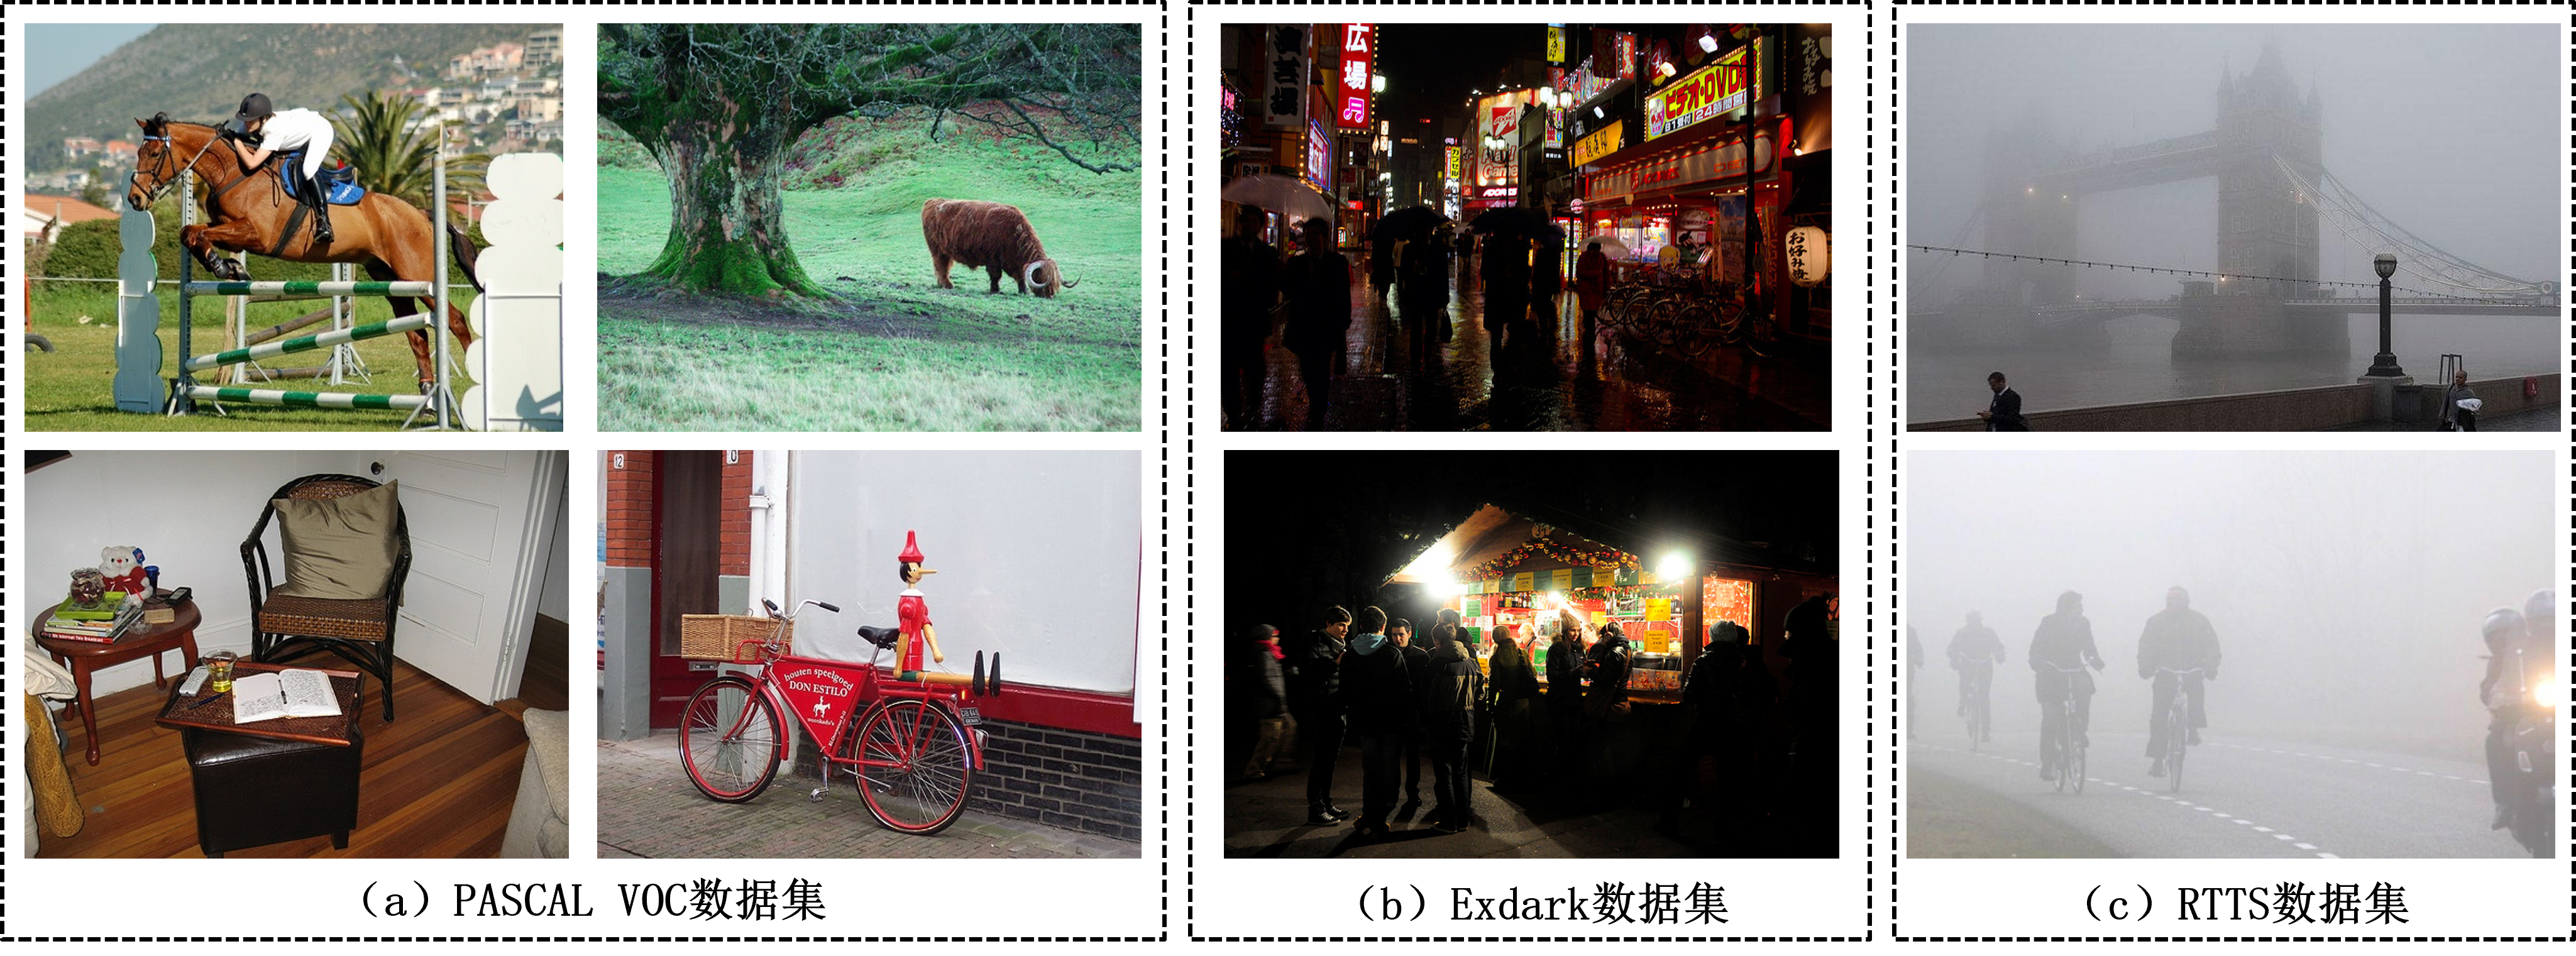
\includegraphics[width=12cm]{chapter1/6.png}
%     \caption{\label{fig:ch1_6}CenterNet算法流程图}
% \end{figure}
在多目标跟踪算法中,FairMOT\cite{fairmot}就是基于CenterNet实现的,其方法非常简洁:额外添加了一个基于卷积层的分支网络,用于生成外观特征图。
该分支网络与CenterNet原有的两个分支网络能并行运行,且相较于主干网络,计算量较小。
具体而言,当某个目标被检测到时,FairMOT根据该目标的中心点,在外观特征图中提取相应位置的特征,作为该目标的外观特征,进而用于后续的轨迹关联步骤。
% \begin{figure}[htbp]
%     \centering
%     \includegraphics[width=12cm]{chapter1/7.png}
%     \caption{\label{fig:ch1_7}FairMOT算法流程图}
% \end{figure}

需要说明的是,随着Transformer\cite{transformer}在计算机视觉任务中的成功,基于Transformer的单阶段检测器也逐渐兴起,如DETR\cite{detr}。
这一进展也推动了多目标跟踪算法的发展。目前已有基于Transformer的单阶段检测器应用到多目标跟踪任务,如TrackFormer\cite{trackformer}。

TrackFormer提出了一种全新的多目标框架——基于Transformer结构统一了目标检测和轨迹关联任务。
具体来说,TrackFormer参考DETR思路,在编码器部分同样使用自注意力机制在特征图上进行全局分析,而在解码器部分,
不仅设计了目标查询(Object Query)来识别和定位潜在目标,还创新性地设计了轨迹查询(Track Query),
通过与目标查询一起的多头自注意力运算来自适应地跟踪目标,从而隐式地完成了轨迹关联。

% \begin{figure}[htbp]
%     \centering
%     \includegraphics[width=15cm]{chapter1/8.png}
%     \caption{\label{fig:ch1_8}TrackFormer算法流程图}
% \end{figure}
\textbf{2. 多目标跟踪中的轨迹关联}
% \subsubsection{多目标跟踪中的轨迹关联}

现有多目标跟踪算法中,最为关键的步骤就是轨迹关联匹配,即轨迹关联。
轨迹关联的核心任务是在检测器生成候选边界框中,将同一目标(或轨迹)对应的边界框赋予一致的身份信息。
根据在轨迹关联过程中是否使用到了未来帧的信息,可分为在线跟踪算法和离线跟踪算法。
在线算法仅依赖当前帧以及历史轨迹的信息进行关联匹配,而离线算法则使用到了多帧甚至全局视频信息进行关联。
在实际关联过程中,首先需要依据轨迹和候选目标的特征信息计算出匹配代价,所以轨迹关联问题的求解本质上是寻找使总匹配代价最小的全局最优匹配方案。

\textbf{(1) 轨迹关联的匹配代价}

在轨迹关联过程中,匹配代价的计算是至关重要的一环。首先,需要从目标中提取具有判别力的特征,主要包括视觉特征与运动特征。
通常情况下,同一目标的视觉特征具有较高的相似性,而不同目标的视觉特征则存在显著差异。
因此,匹配代价的计算通常由视觉特征之间的余弦距离和目标边界框之间的交并比共同构成。
此外,近年来也有研究者提出通过深度神经网络,将目标的视觉特征与运动特征作为输入,
直接学习目标的匹配代价矩阵,以优化关联过程。这种基于学习的方法能够在特征提取与匹配代价计算之间实现更紧密的融合,
从而提升多目标跟踪的整体性能。

\begin{figure}[htbp]
    \centering
    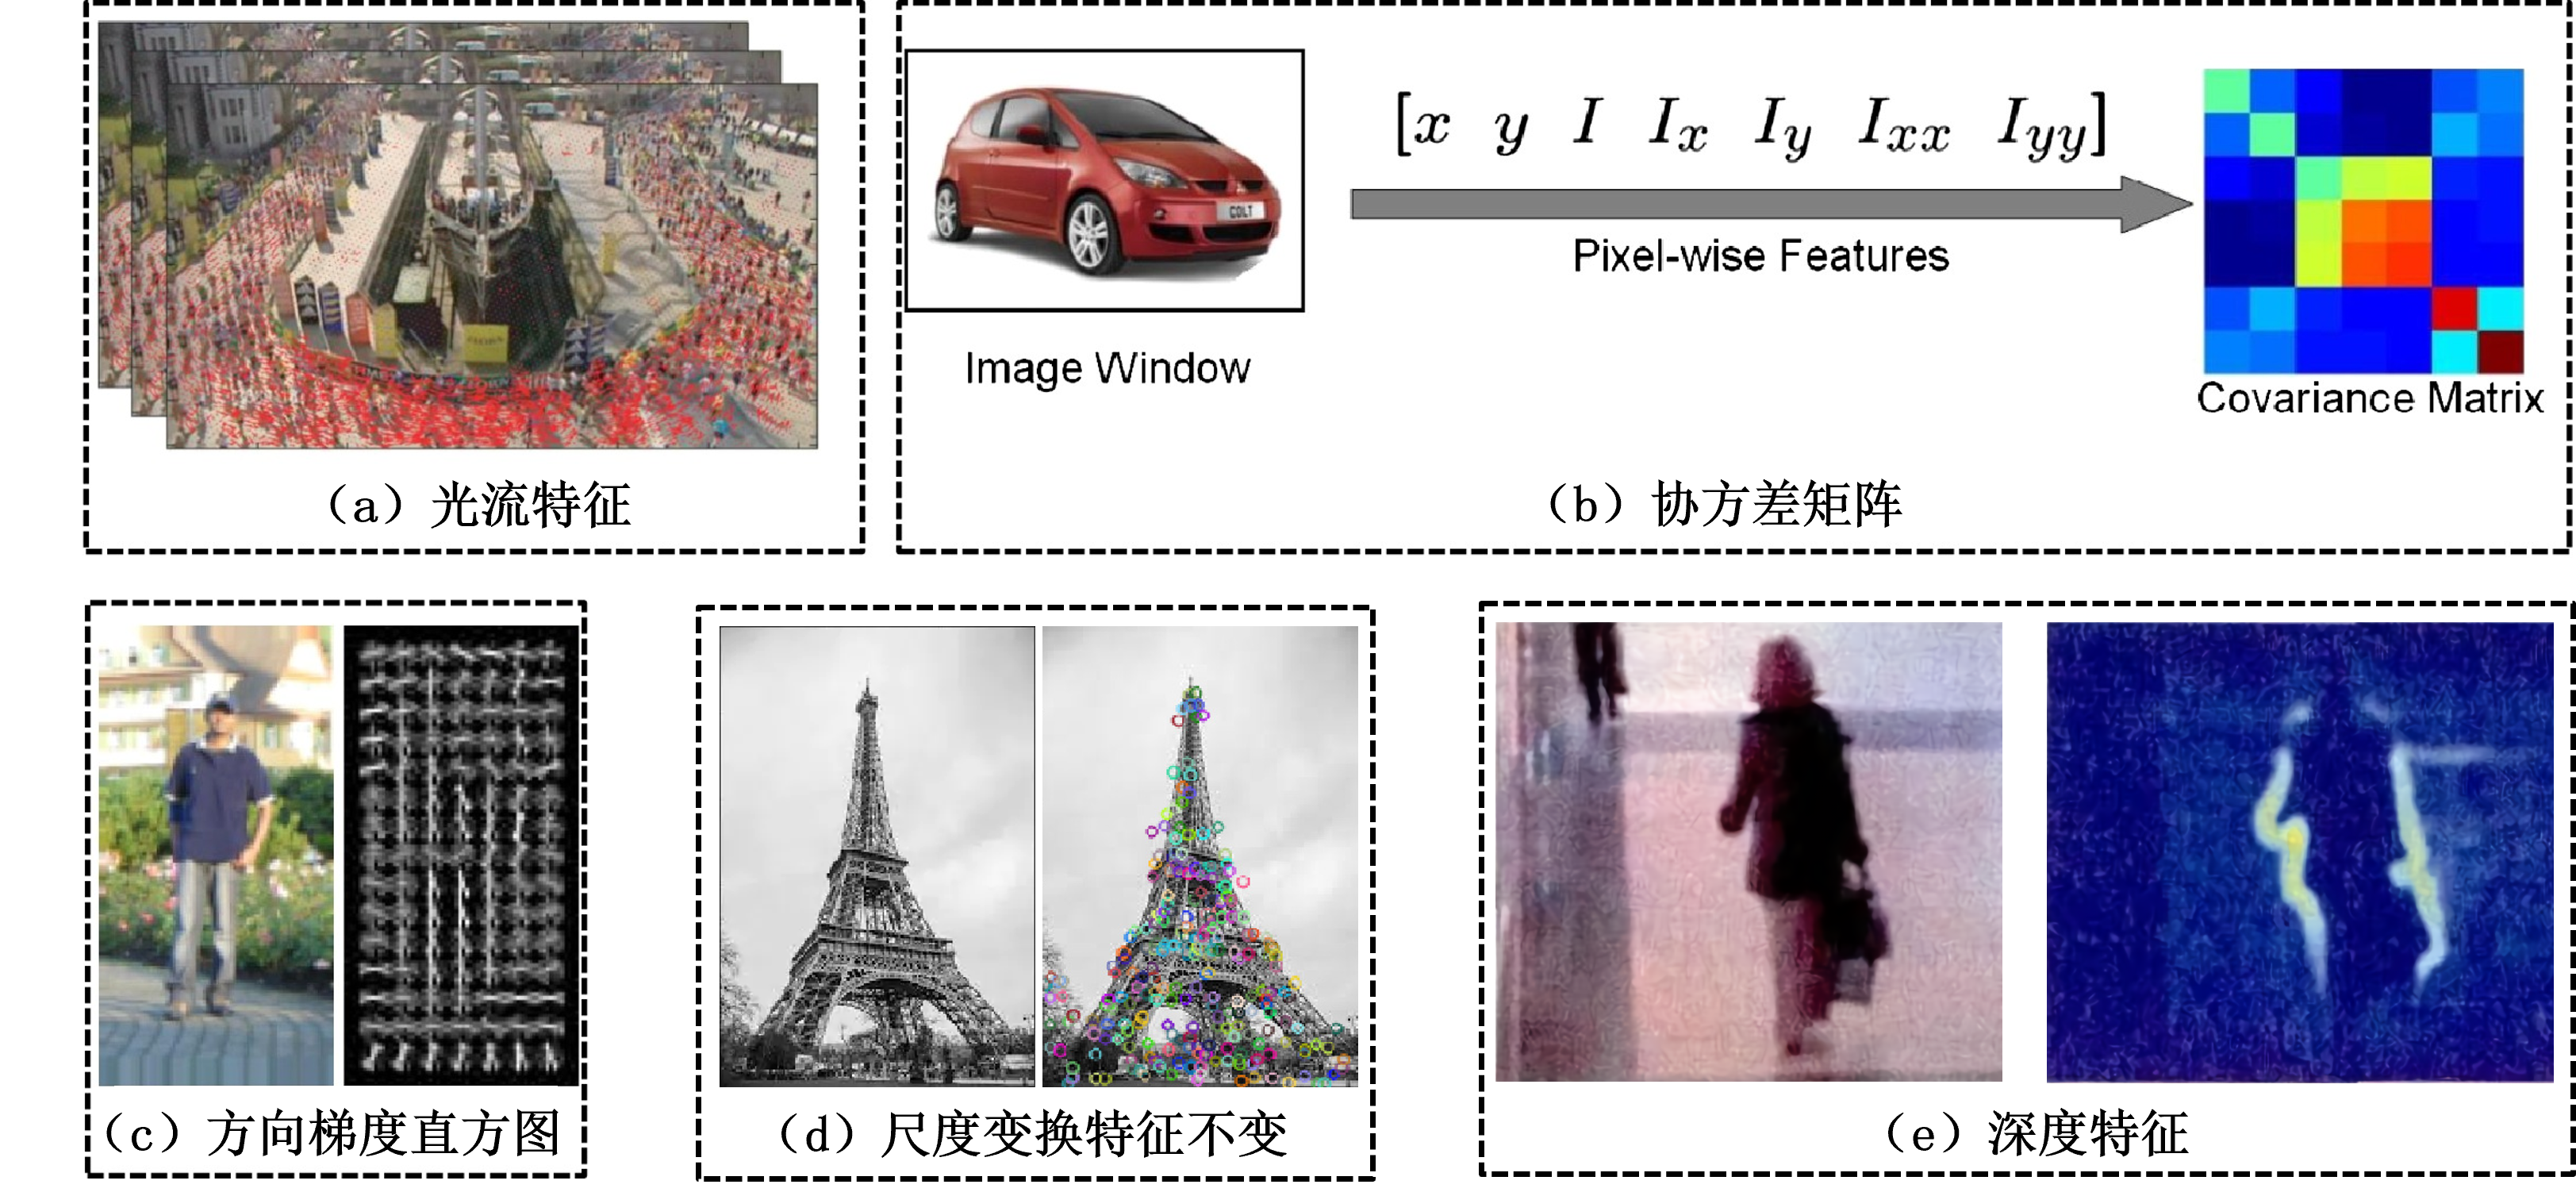
\includegraphics[width=15cm]{chapter1/9.png}
    \caption{\label{fig:ch1_9}视觉特征}
\end{figure}
视觉特征用来描述目标的外观信息,通常分为传统特征与基于深度学习的特征。
传统特征包含光流、协方差矩阵、尺度不变特征变换(Scale-Invariant Feature Transform,SIFT)\cite{sift}、方向梯度直方图特征(Histogram of Oriented Gradients,HOG)等。
光流特征基于图片亮度模式的变化来表征目标运动信息,协方差矩阵能够融合多种类型的特征,而SIFT与HOG特征的在计算机视觉领域应用广泛。
SIFT 特征的核心思想是在多尺度空间上检测关键点并计算其方向,这些关键点通常为角点、边缘点、暗区亮点或亮区暗点等,
在光照、仿射变换和噪声干扰下仍具备稳定性。SIFT特征具有尺度、旋转和仿射不变性,能够有效应对目标旋转、缩放及光照变化问题。
其次,HOG特征通过计算局部区域的梯度方向直方图,统计梯度或边缘的方向密度分布,从而描述目标的外观与形状特征。
近年来,基于深度学习的特征提取方法也逐渐应用到多目标跟踪任务中。如Yu等人\cite{yu2016poi}对GoogleNet\cite{googlenet}网络结构进行修改,
并在行人重识别数据集上训练用以提取表观特征;Wojke等人\cite{deepsort}在SORT模型基础上引入了深度残差网络作为表观特征提取器,
提出了DeepSORT模型。

运动特征用来描述目标在轨迹中的位置、速度及运动方向等信息,通常分为线性运动模型和非线性运动模型。线性运动模型假设目标在空间保持匀速运动,
一般通过卡尔曼滤波器(Kalman Filter)\cite{kf}来估计目标的运动速度。
它考虑到观测到的目标位置框中存在噪声,所以先对当前帧的目标进行预测,估计其在下一帧中的位置框,
然后根据预测的边界框与下一帧的检测框计算匹配代价。在完成轨迹关联匹配后,使用匹配到的检测框再对卡尔曼滤波器进行更新。
然而,由于线性运动模型过于简单难以准确描述目标在复杂场景下的位置,因此研究人员在多目标跟踪任务中引入非线性模型。
如Sadeghian等人\cite{untrackable}基于长短时记忆网络(Long Short Term Memory,LSTM)\cite{lstm}设计了非线性运动模型,通过输入目标的历史轨迹坐标,学习并预测相似的运动模式,
最后输出高维的特征向量。 

\textbf{(2) 轨迹关联的优化算法}

从多目标跟踪任务的特点来看,短期内轨迹关联可认为是偶图匹配问题,而长期上来看则可建模为网络流问题。
因此,在在线跟踪算法中,常用的匹配优化算法是匈牙利算法(Hungarian Algorithm)\cite{hungarian},
而离线跟踪算法中通常使用的匹配优化算法包括最小代价网络流算法等。

\begin{figure}[htbp]
    \centering
    \includegraphics[width=15cm]{chapter1/10.png}
    \caption{\label{fig:ch1_10}轨迹关联算法示意图}
\end{figure}
匈牙利算法是一种在多项式时间内求解无边权二分图最大匹配的组合优化算法。
美国数学家库恩(W.W.Kuhn)于1955年利用匈牙利数学家康尼格(D.Kőnig)的一个定理构造了这个算法,故称为匈牙利算法。
匈牙利算法的实现较为成熟,它的核心思想是先选定一条初始的匹配方法,然后逐步寻找它的增广路径,最终达成了最大匹配。
SORT和Deep SORT都使用了匈牙利算法来实现轨迹关联,因其简单有效的跟踪流程成为了后续大量算法的基础(baseline)。

网络流是一种带有边容量约束的有向图。在多目标跟踪任务中,图的节点通常表示检测结果或历史轨迹,而流被建模为连续两个节点间的关系。
为了满足流量守恒约束,分别对应轨迹的初始帧与结束帧的源点(Source Node)和汇点(Sink Node)被添加到图中。
其中,一条轨迹可视为图中一条流动路径,从源点到汇点的总流量数目等于轨迹总数。
Zhang等人\cite{zhang2008global}首先将网络流模型引入到多目标跟踪任务的轨迹关联问题中,
将最大后验概率轨迹关联问题映射为具有非重叠约束的轨迹成本流网络中,并通过最小成本流算法求解最佳轨迹关联方案。

\subsection{图神经网络在多目标跟踪中的应用}
\label{subsec:gnn_apply}
多目标跟踪中的轨迹关联问题本质上可以抽象为图结构建模问题,其核心在于刻画检测目标与历史轨迹之间的关联关系。
然而,传统的轨迹关联方法大多依赖不可学习的优化策略,在动态复杂环境中难以充分建模目标之间的复杂关系,且无法实现端到端优化,
容易导致误差在时序上的累积。此外,由于目标在视频中的出现时长不一致,其对应轨迹数据通常具有长度不固定、结构不规则等特点,
这进一步增加了轨迹关联建模的难度。

图神经网络(Graph Neural Network,GNN)在非结构化数据建模和关系推理方面具有显著优势,能够自然地处理变长轨迹和复杂交互关系。
得益于这一特性,近年来越来越多的研究尝试将图神经网络引入多目标跟踪中的轨迹关联任务,以提升关联精度并降低训练与推理成本。
围绕轨迹关联的时序处理方式,这类方法逐渐形成了在线跟踪与离线跟踪两种主要研究方向,下面将分别进行介绍。

\textbf{1. 基于图神经网络的在线跟踪算法}

GNMOT\cite{li2020graph}将多目标跟踪中的二分图匹配问题建模为图神经网络中的边分类任务。
该方法分别利用图神经网络对目标的表观特征和运动特征进行建模,并在此基础上融合两类信息以构建目标与轨迹之间的相似度矩阵,
从而完成轨迹关联过程。此外,GNMOT在图神经网络结构中引入了全局节点,
用于在消息传递过程中提供全局上下文信息,以增强不同节点之间信息交互的协调性。

% \begin{figure}[htbp]
%     \centering
%     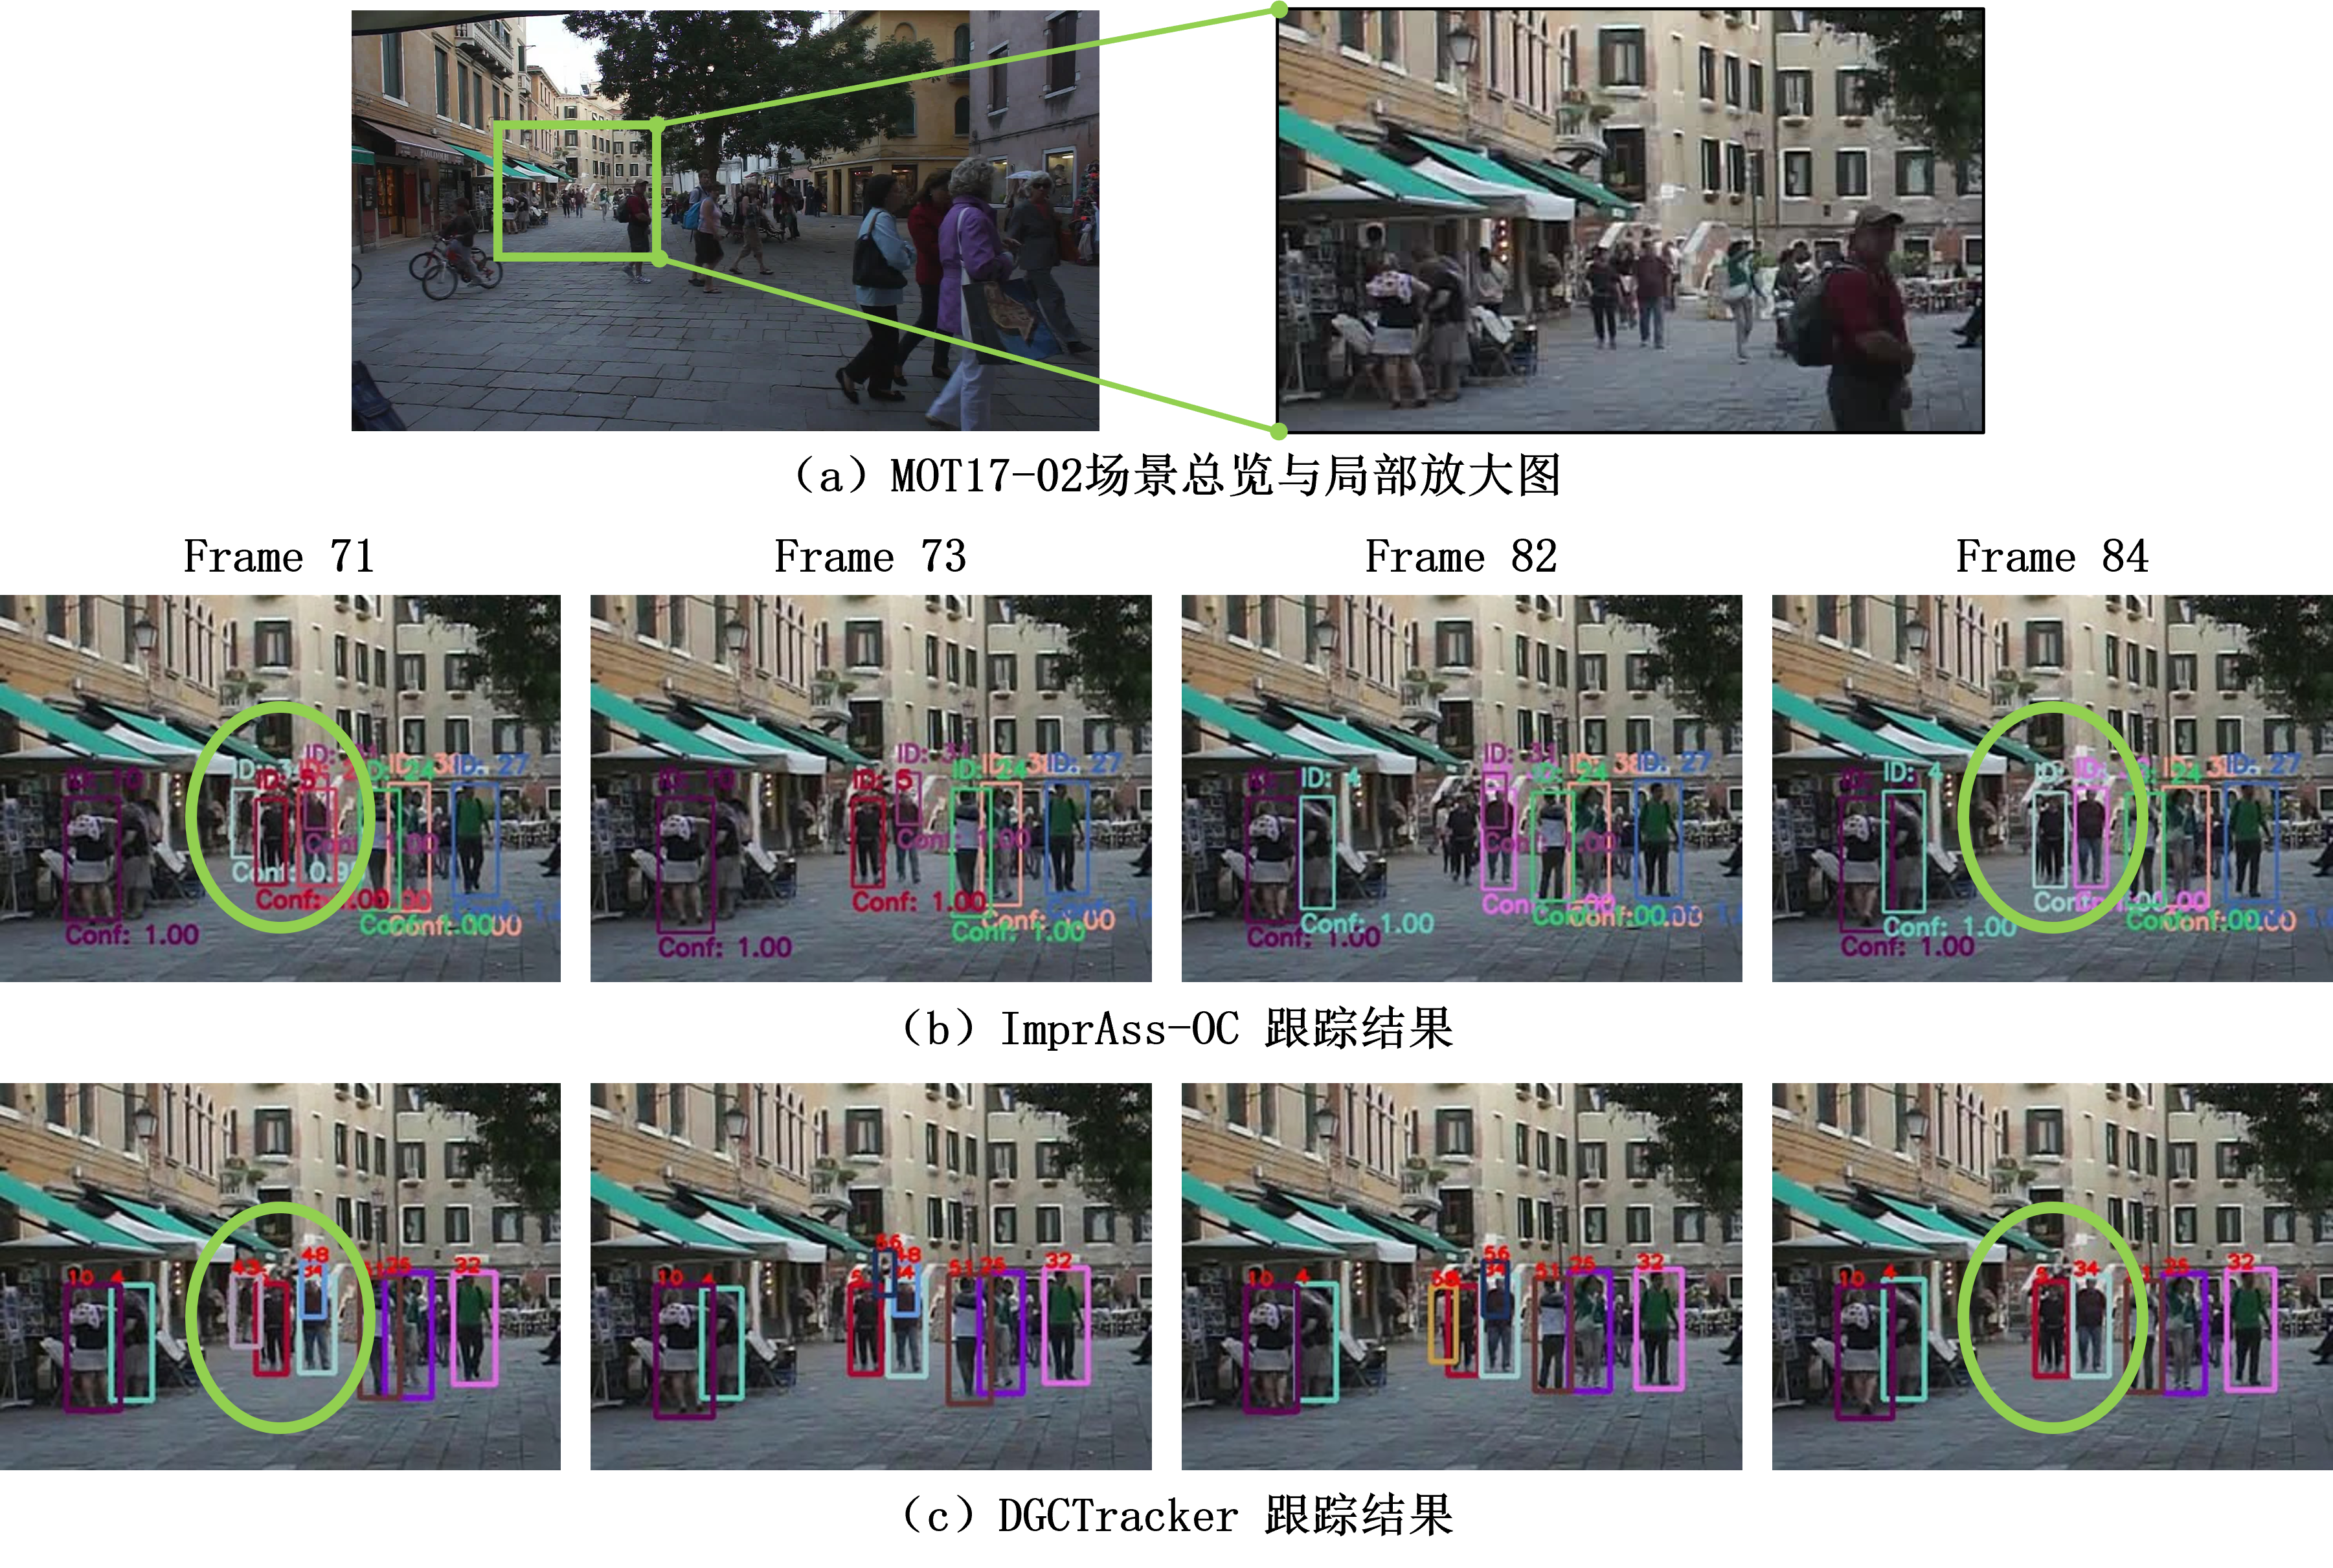
\includegraphics[width=15cm]{chapter1/12.png}
%     \caption{\label{fig:ch1_12}GNMOT算法流程图}
% \end{figure}
GNN3DMOT\cite{weng2020gnn3dmot}通过融合视觉信息与雷达点云信息来提升轨迹关联的匹配效果。而且与GNMOT直接构建全连接图不同,
GNN3DMOT引入了节点之间的空间距离约束,仅将相邻两帧中位于相近图像空间内的节点进行连接,从而简化了图模型的复杂度。
这种方式不仅减少了冗余连接,还有效提升了匹配的准确性和计算效率。TransMOT\cite{chu2023transmot}同样利用了空间距离约束,
但其创新之处是将同一帧中的各个物体边界框的交并比来定义边,并以交并比的值作为边权,完成了图的构建。
此外,TransMOT还创新性地设计了Graph-Transformer结构来提取检测目标和轨迹的时空信息,从而更有效地指导轨迹关联匹配。

% \begin{figure}[htbp]
%     \centering
%     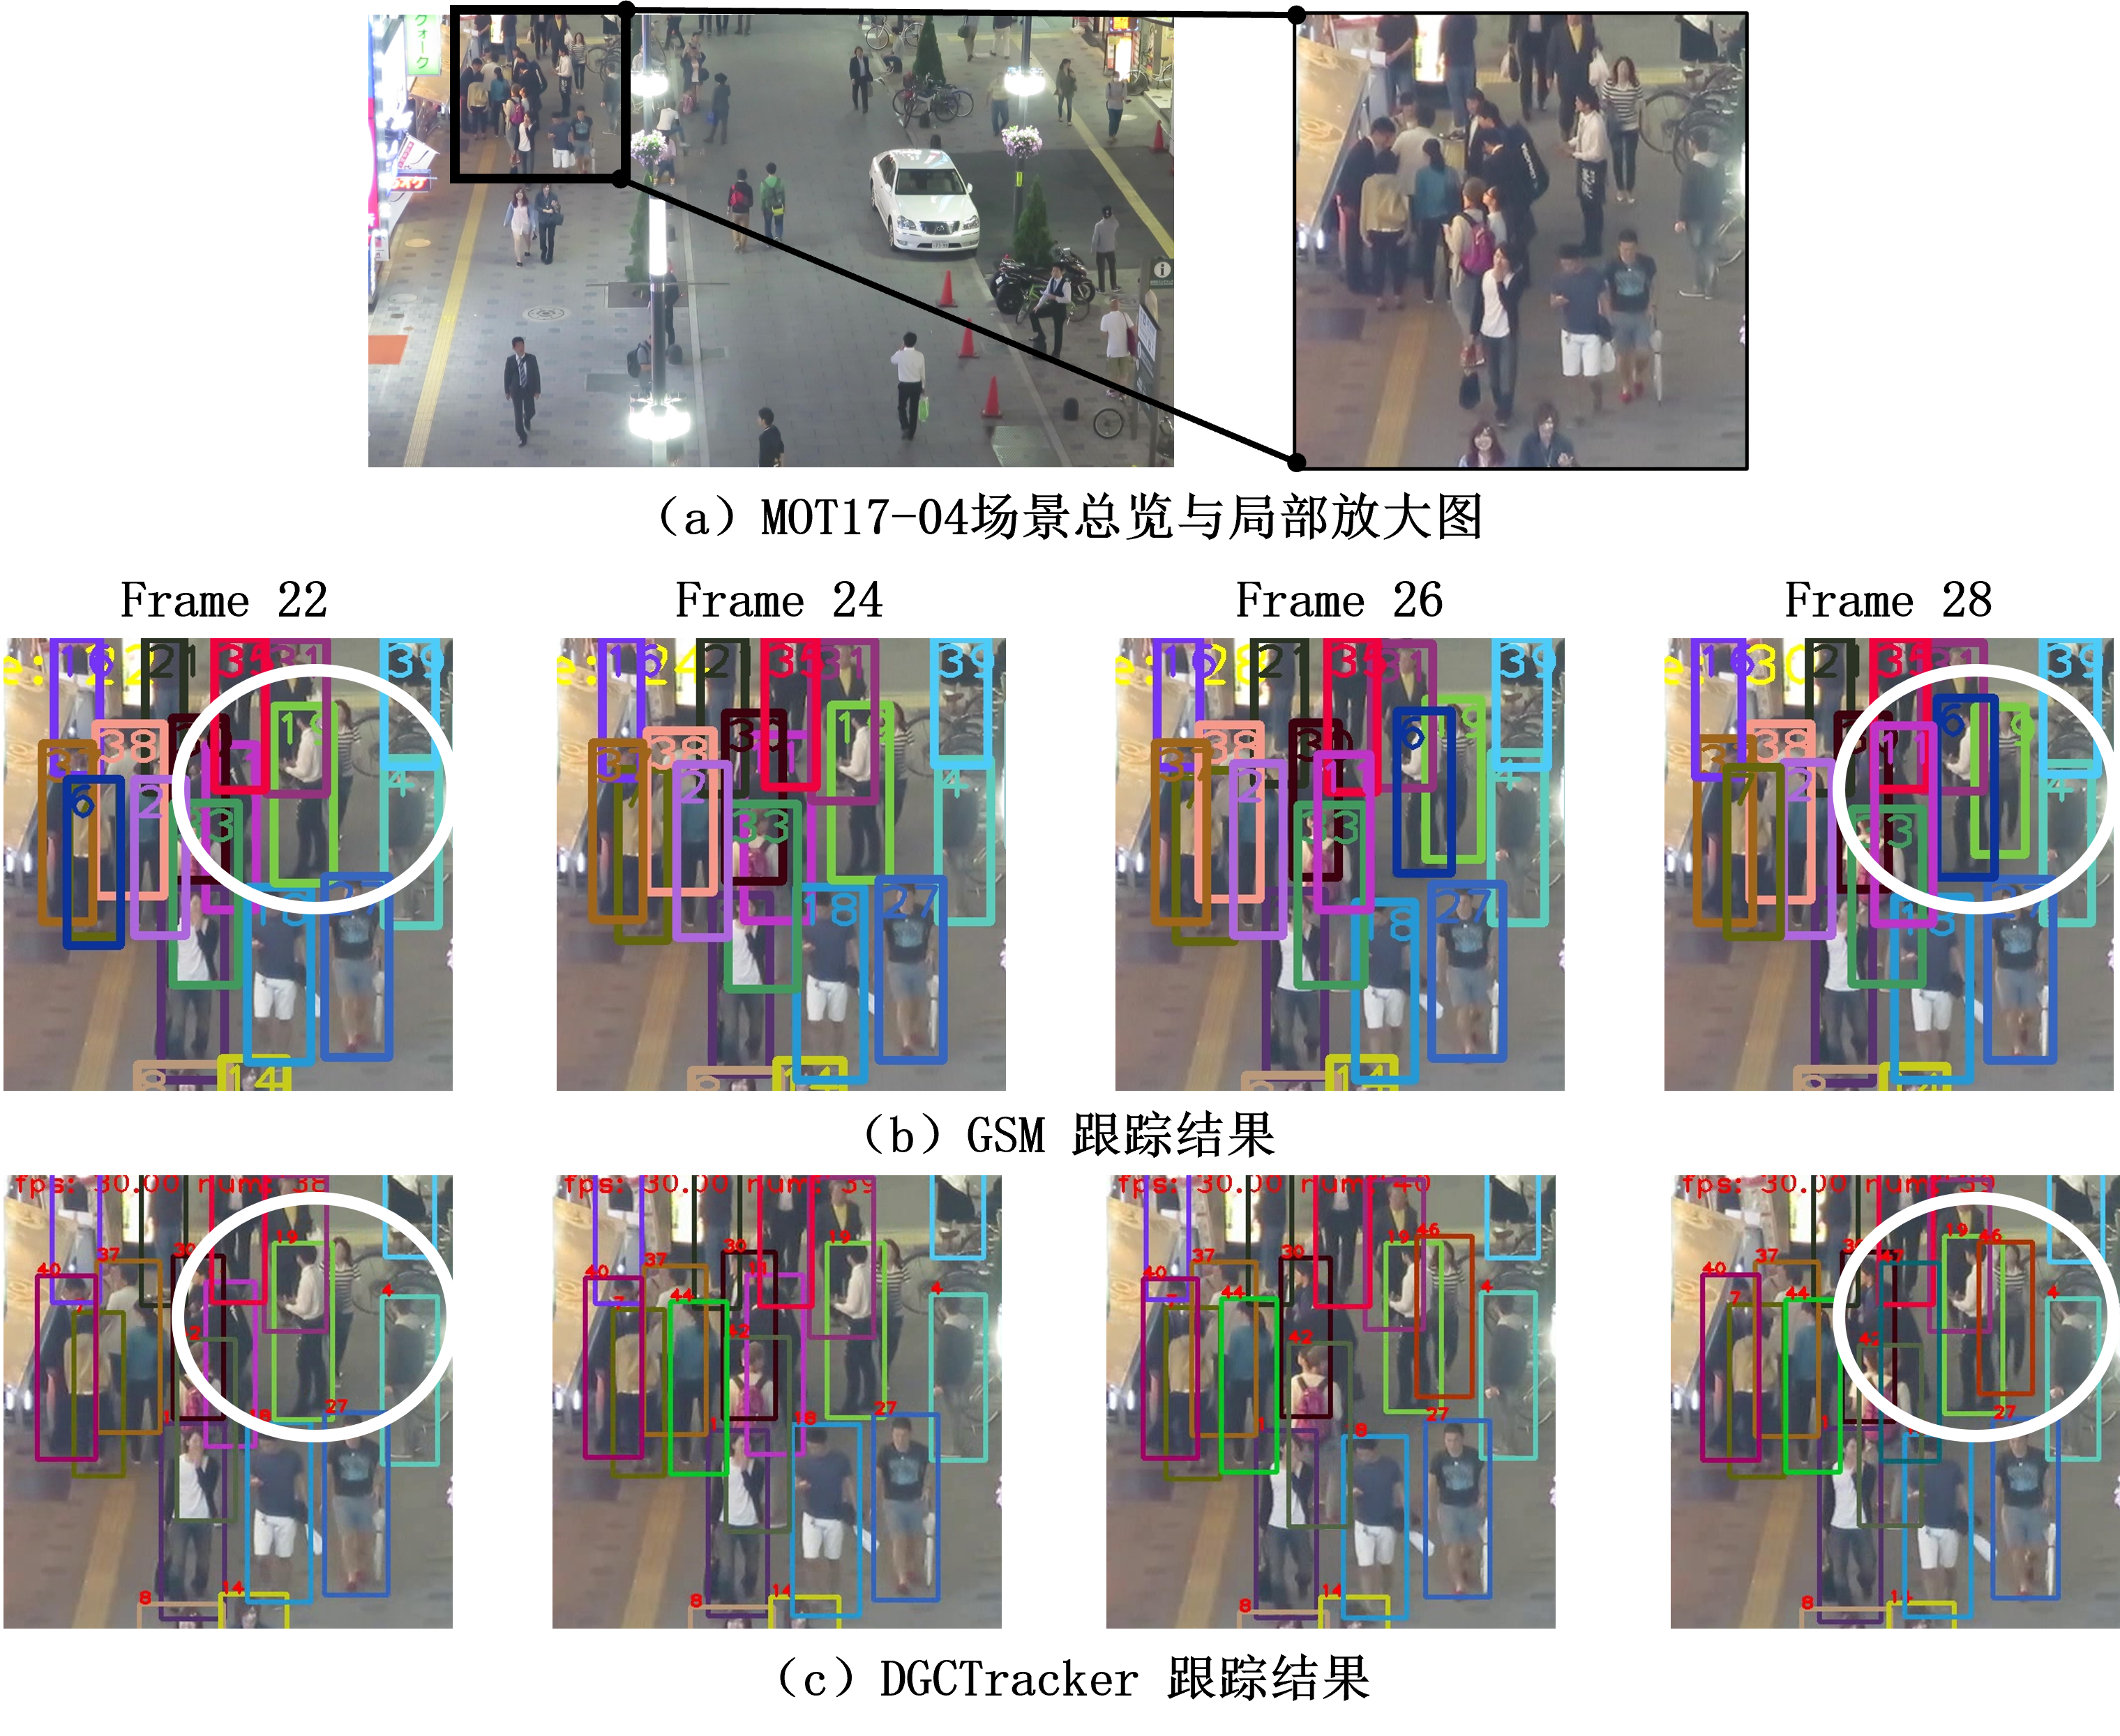
\includegraphics[width=12cm]{chapter1/13.png}
%     \caption{\label{fig:ch1_13}TransMOT算法流程图}
% \end{figure}
上述方法均从损失函数的设计角度出发,以满足二分匹配的约束,而GCNNMatch\cite{gcnnmatch}则通过Sinkhorn\cite{sinkhorn}最优传输算法对相似度矩阵进行优化,以实现轨迹与目标之间的一对一匹配约束。
这种方法使得在训练阶段和推理阶段能够一致性处理,从而提高了跟踪精度。
此外,GCNNMatch仅利用图神经网络提取轨迹和目标的特征,并结合位置信息来构建相似度矩阵,从而增强了匹配的准确性和鲁棒性。

% \begin{figure}[htbp]
%     \centering
%     \includegraphics[width=15cm]{chapter1/14.png}
%     \caption{\label{fig:ch1_14}GCNNMatch算法流程图}
% \end{figure}
与上述方法不同,GMTracker\cite{gmtracker}将轨迹关联问题视为图之间的一般图匹配问题。
具体而言,GMTracker将轨迹和当前检测的目标都视作节点,分别构建得到全连接的轨迹图和检测图,
并通过ReID网络提取外观特征来初始化节点嵌入。之后,作者设计了跨图的图卷积网络,
利用轨迹图和检测图之间的结构亲和信息对节点嵌入进行增强,从而得到节点间和边间的相似度矩阵。
并且作者借鉴OptNet\cite{amos2017optnet}的思路构建了一个可微分的二次规划优化层,来求解图匹配问题,完成轨迹关联。
实验结果表明,GMTracker在处理遮挡等复杂情况时,比仅基于节点间一阶相似度的二分图匹配算法具有更高的鲁棒性。

% \begin{figure}[htbp]
%     \centering
%     \includegraphics[width=12cm]{chapter1/15.png}
%     \caption{\label{fig:ch1_15}GMTracker算法流程图}
% \end{figure}
上述算法大多遵循基于检测的跟踪范式,即将目标检测与轨迹关联作为相对独立的模块进行处理。
由于检测算法与关联算法之间存在明显分离,在整体优化过程中对各模块之间的协同与融合提出了较高要求,
容易出现局部最优和误差累积等问题。同时,分离式结构在特征提取与表示层面往往存在一定冗余,
限制了模型的整体效率。
基于此,近年来有研究尝试引入图神经网络等关系建模方法,对检测目标与历史轨迹之间的关联关系进行统一建模,
从而推动检测模块与轨迹关联模块的深度融合,构建联合检测与跟踪框架,如GSDT\cite{wang2021joint}.

GSDT算法在FairMOT基础上,利用图卷积结合检测器,构建了一个端到端的多目标跟踪网络。
具体来说,将轨迹以及空间上邻近的检测特征点作为节点构建全连接图,并在外观特征提取的过程中引入历史信息,提高算法鲁棒性。

SGT\cite{hyun2023detection}算法同样采用图卷积网络结合检测器的方式来进行检测和跟踪。从跟踪面临的遮挡、检测缺失等问题出发,
在轨迹关联过程中对类别置信度高的检测目标和轨迹(包括因丢失目标而中断的轨迹和正活跃的轨迹)都视为节点,
依据表观相似性和空间相似性来有选择地建立连边,以外观特征作为节点嵌入,相对空间距离作为边嵌入,从而完成了稀疏二分图的搭建。
最后通过图神经网络来对边进行分类,从而完成了轨迹关联匹配。

% \begin{figure}[htbp]
%     \centering
%     \includegraphics[width=12cm]{chapter1/16.png}
%     \caption{\label{fig:ch1_16}SGT算法流程图}
% \end{figure}
\textbf{2. 基于图神经网络的离线跟踪算法}

MPNTracker\cite{MPNTracker}是一种利用图神经网络对传统网络流进行建模的离线跟踪算法。
具体而言,给定一段视频序列,在前端检测器检测出视频中的所有目标之后,MPNTracker将每个检测到的目标表示为图中的节点,
并通过卷积神经网络提取其表观特征,以此作为节点的初始嵌入。接着,将边定义为两个相邻目标之间的潜在匹配关系,
并将节点间的相对表观特征和时空距离编码作为边的初始嵌入。通过这种方式,图结构得以构建,
使得轨迹关联与匹配问题可以转化为一个边的二分类问题——即判断相连的两个目标是否属于同一条轨迹。
MPNTracker中图的定义简单直观,通过构建全局完全图,使得其在保持跟踪目标身份一致性方面表现优异。
然而,由于完全图中包含了过多冗余边,导致网络存储开销大、推理效率较低。

% \begin{figure}[htbp]
%     \centering
%     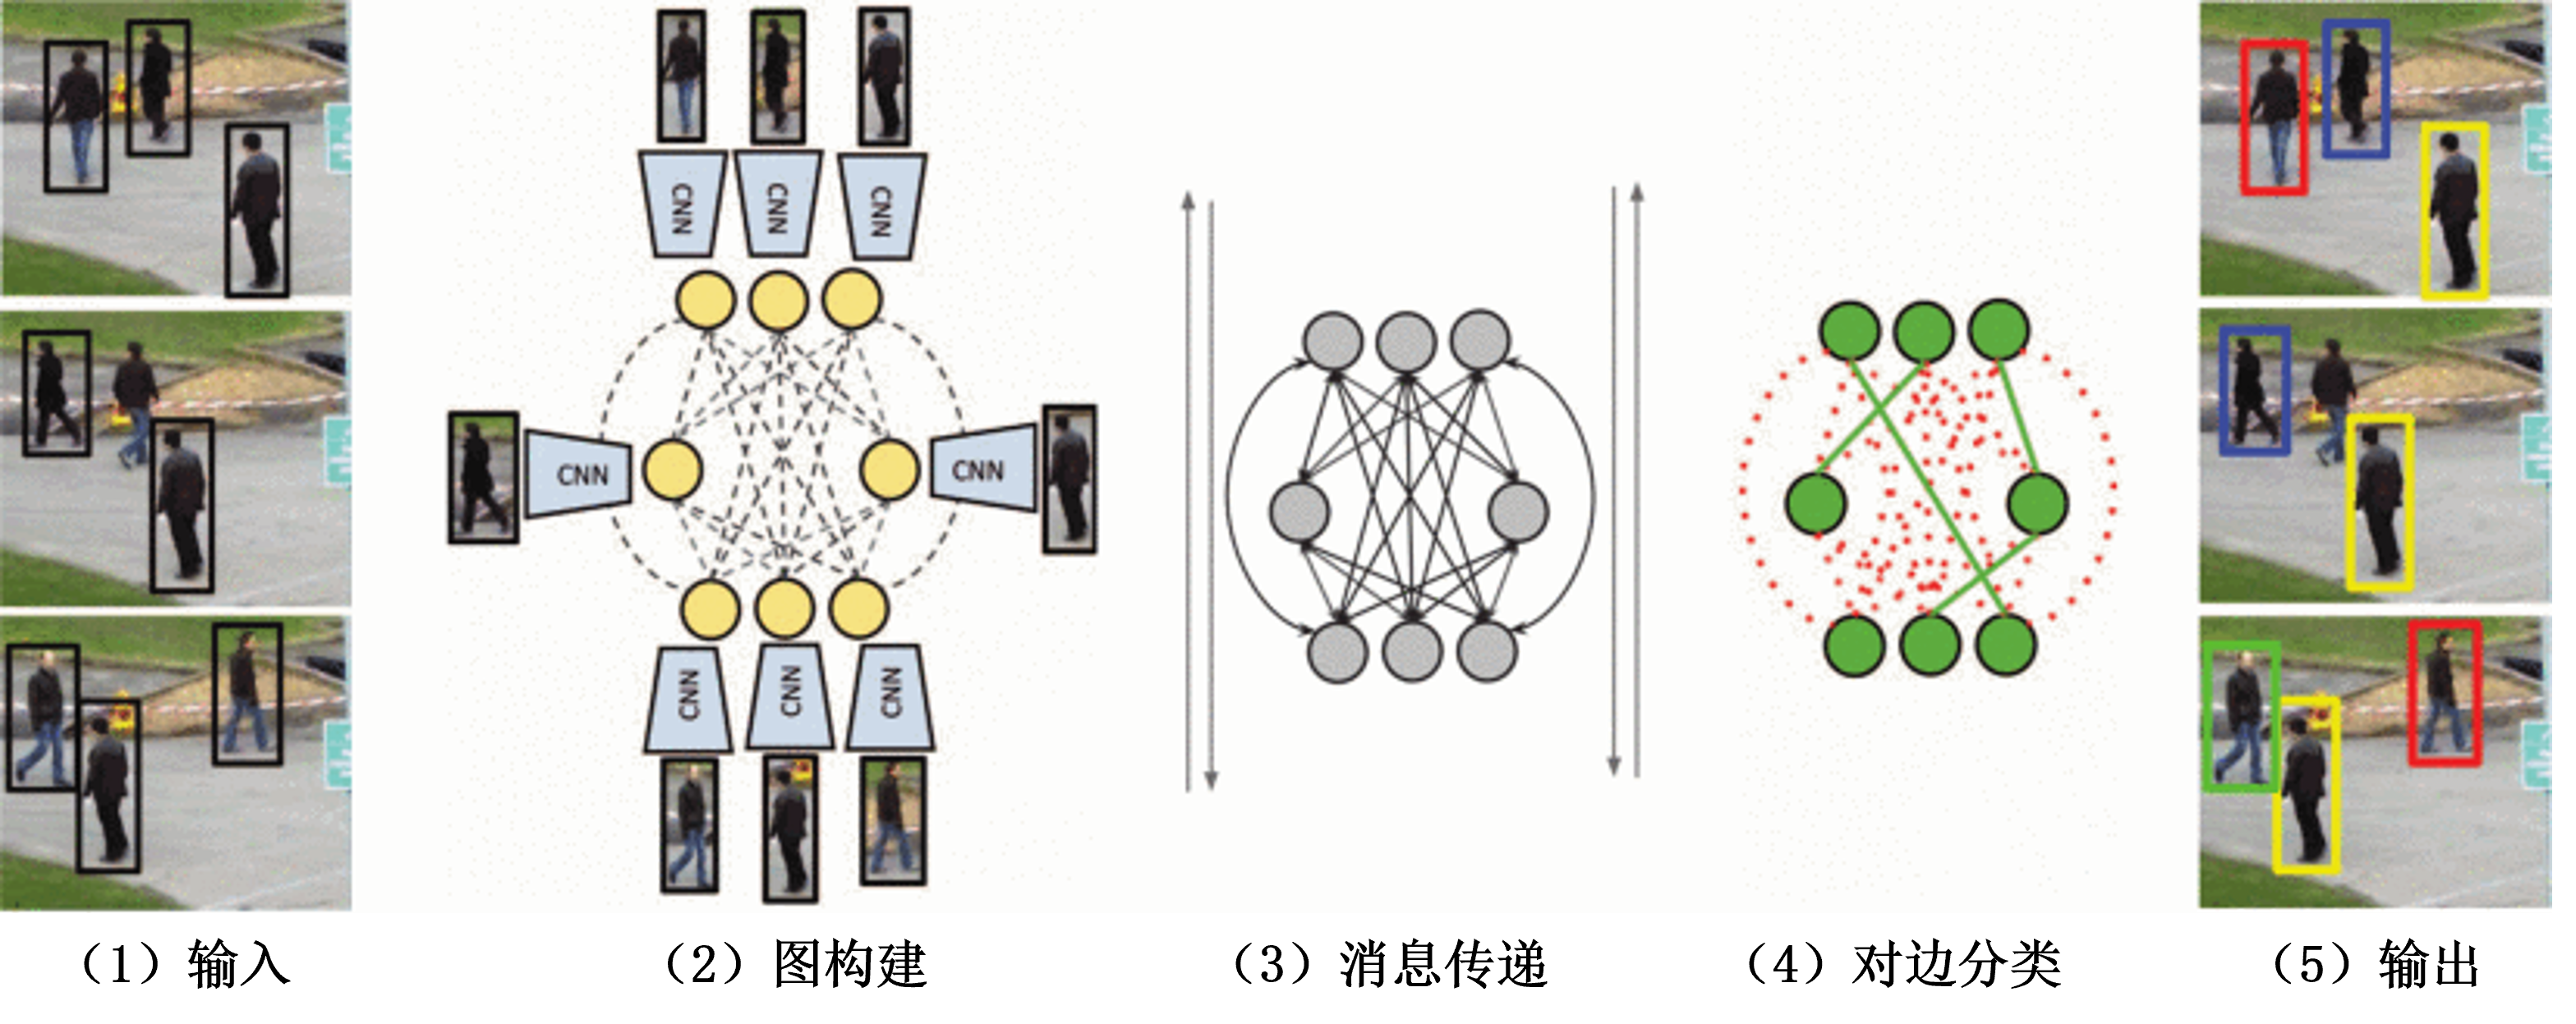
\includegraphics[width=15cm]{chapter1/17.png}
%     \caption{\label{fig:ch1_17}MPNTracker算法流程图}
% \end{figure}
针对上述问题,SUSHI\cite{sushi}提出了一种层级递归式图关联方法。具体而言,对于给定的视频序列,
SUSHI首先在不重叠的时间窗口内按照MPNTracker的图结构定义构建子图,并对边进行分类任务。
接着,在更大时间范围内,将初步得到的小轨迹合并为更长的轨迹,基于此构建跨时间段的更大图结构,
此时新的节点代表合并后的轨迹。通过这种方式,SUSHI建立了多层次的图结构,并递归地实现全局轨迹关联。

为进一步对图结构进行稀疏化,Gao等人\cite{gao2024multi}将检测目标和轨迹均视为图中的节点,并设计了基于Transformer结构的NodeNet网络。
在滑动时间窗口内,NodeNet选择性地连接潜在可能匹配的目标,并将每个时间窗内的第一帧检测目标也初始化为轨迹节点。
在构建出初步的稀疏图后,利用图神经网络对其进行进一步细化处理——在同一时间窗内,检测节点与下一个相同目标的检测节点关联,
并连接到表征该目标的轨迹节点,形成各个目标的短轨迹;轨迹节点则在跨时间窗内与同样表征相同目标的轨迹节点相连,从而实现短轨迹的逐步融合,
形成更长的轨迹。实验结果表明,该方法在计算复杂度、显存占用方面都优于SUSHI模型,并且在MOT17\cite{mot16}基准数据集上表现显著提升,
关键的跟踪指标都突破了80\%。
\subsection{跨域视觉感知与自适应方法研究}
\label{subsec:cross_domain}
尽管上述小节介绍的多目标检测与跟踪方法已经在许多数据集上表现出了越来越好的结果,但在开放世界的实际部署中,
多目标跟踪系统不可避免会遭遇训练数据(源域)与测试环境(目标域)之间的分布偏移,即域差异问题。
如\autoref{fig:ch1_18}所示,光照剧变、恶劣天气(如雾、雨)等导致的低级视觉外观变化,会严重退化检测器与特征提取器的性能,
进而破坏整个跟踪链路的可靠性。因此,研究跨域视觉感知与自适应方法,对于提升多目标跟踪系统的环境鲁棒性与泛化能力至关重要。
\begin{figure}[htbp]
    \centering
    \includegraphics[width=12cm]{chapter1/18.png}
    \caption{\label{fig:ch1_18}跨域条件下视觉外观差异示例}
\end{figure}

目前,针对跨域适应问题,研究者们提出了多种方法。传统的域适应方法主要依赖于特征对齐或生成式方法,通过缩小源域与目标域之间的分布差异来实现
跨域的感知与自适应。然后,这些方法通常面临着特征对齐困难和生成图像质量受限的问题。为了解决这些挑战,近年来,一些前端自适应增强的方法开始受到
关注。该方法通过自适应地改善输入图像质量,从源头缓解底层视觉退化,为下游任务提供了更鲁棒的视觉前端。为系统梳理该领域的研究脉络,本节将依次对上述
三类方法进行介绍与评述。

\textbf{1. 基于特征对齐的域适应方法}

此类方法旨在通过在特征空间中对齐源域与目标域的分布,以学习对域变化不敏感的特征表示。其中,基于对抗学习(Adversarial Learning)的范式因其有效性与可拓展性而成为主流实现方式之一。其理论基础源于Ben-David等人
提出的域适应理论\cite{ben2010theory},并由Ganin等人\cite{ganin2016domain}开创性地通过梯度反转层实现了端到端训练。

Ganin等人工作的核心目标是使特征提取网络$F$能够产生域不变特征,即让后续的域分类器$h$无法有效判断特征来源于源域还是目标域。这被建模成一个极小极大优化问题:特征提取器$F$需在最小化特定任务(如分类、检测等)的损失的同时,最大化域分类器$h$的损失(即欺骗域分类器);而域分类器$h$则需最小化自身的域分类误差。
这一对抗性目标可形式化表示为:
\begin{equation}
    \label{equ:loss_h}
    \min_F \max_{h\in\mathcal{H}}{\lbrace \mathbb{E}_\mathcal{S} \lbrack L_h\rbrack + \mathbb{E}_\mathcal{T} \lbrack L_h\rbrack \rbrace}
\end{equation}
其中,$\mathcal{H}$表示域分类器的假设空间,$\mathbb{E}_\mathcal{S}$和$\mathbb{E}_\mathcal{T}$分别表示源域和目标域的期望损失。具体流程如\autoref{fig:ch1_19}所示。其中梯度反转层在正向传播中作为恒等映射,而在
反向传播时将梯度乘以负系数,从而巧妙的在一个前向-反向过程中实现了特征提取器与域分类器的对抗性训练。

\begin{figure}[htbp]
    \centering
    \includegraphics[width=15cm]{chapter1/19.png}
    \caption{\label{fig:ch1_19}基于梯度反转层的域对抗训练框架}
\end{figure}

为提升特征对齐的精细度与鲁棒性,后续研究从不同角度对基础的梯度反转训练进行了改进。例如,Zheng等人\cite{zheng2020cross}针对检测任务中多尺度目标的特点,在特征金字塔的多层上应用域分类器,
并利用通道注意力权重动态调整各层对抗损失的贡献,实现了多尺度、有重点的特征对齐。对于多分类场景,VS等人\cite{vs2021mega}发现不同类别的特征可能发生错位,因此提出通过记忆网络生成类别特定的注意力图,
以引导模型进行更精确的类内特征对齐,同时避免了类间干扰。此外,针对单阶段检测器的效率需求,Zhang等人\cite{dayolo}在DA-YOLO中设计了图像级与实例级的多层次对齐策略,并辅以一致性正则化,有效提升了YOLO架构
在跨域场景下的检测性能。

\textbf{2. 基于图像翻译的生成式方法}

与在特征空间进行隐式对齐的思路不同,基于图像翻译的生成式方法尝试在像素层面直接缓解域差异。该方法通过训练一个图像转换模型(如生成对抗网络)来操纵图像风格,以应对域偏移问题。

\textbf{(1) 目标域转换到源域}。其核心目的是将目标域图像(如雾天、夜间)的风格转换为源域风格(如晴天、白天),从而在输入层面“消除视觉外观”的分布偏移。经过转换的
类源域图像能够直接适配在清晰数据上预训练好的检测器,使其能够在不进行大规模重训练或结构调整的情况下,获得对新环境的初步适应能力。例如,Hsu等人\cite{hsu2020progressive}提出了一种渐进式域自适应策略,首先利用基于CycleGAN\cite{cyclegan}的图像转换模块
将目标域图像转换为类源域图像,随后在特征空间进一步对齐残留的域差异,从而有效缓解了直接跨域带来的性能下降问题。

\textbf{(2) 源域转换到目标域}。其本质就是一种面向域差异的数据增广策略。通过将源域数据(通常带有丰富标注)转换为模拟目标域风格的图像,该方法能够有效扩充和多样化训练集,使模型能够在训练阶段就能接触到
更广泛的域变化,从而学习到对风格干扰更鲁棒的特征表示。例如,Arruda等人\cite{arruda2019cross}利用图像转换模块将白天的源域数据转换为“模拟夜间”图像,并利用其真实标签监督训练检测器,从而学习对夜间场景更适应的特征。

然而,这类生成式方法存在固有局限。其转换过程本质上学习两个图像集合之间的整体风格映射,难以精确控制语义属性的转换,容易在生成图像中引入与场景语义不符的伪影或内容。如\autoref{fig:ch1_20}所示,在将暗光场景转换到亮光域时,模型错误将人物区域添加绿色的植物叶子;而将亮光场景转换到
暗光域时,模型又机械地叠加暗光域的典型噪声(如为天空的云彩不合逻辑地添加光斑和光晕)。这种因无法精确控制语义而过拟合目标域表象或引入伪影的现象,会损害生成图像的语义一致性与真实性,进而可能误导下游检测与跟踪模型,导致其在跨域场景中的性能下降。

\begin{figure}[htbp]
    \centering
    \includegraphics[width=15cm]{chapter1/20.png}
    \caption{\label{fig:ch1_20}生成式方法在跨域转换中的语义不一致性示例}
\end{figure}

\textbf{3. 基于前端自适应增强的方法}

针对生成式图像转换方法在参数规模与实时性上的局限性,近期研究转向轻量化、可微分的前端自适应增强策略,通过直接在检测器流水线中嵌入图像增强模块,实现对输入
图像的实时自适应处理。此类方法无需依赖复杂的生成模型,而是通过设计可学习的图像处理滤波器,在保持低计算开销的同时,动态调整图像特征以适应下游检测任务的需求。

IA-YOLO\cite{ia}首次提出了将传统图像处理操作转换为可微模块的思想。其核心在于引入一个参数预测网络,通过小型卷积神经网络动态估计去雾、白平衡、伽马矫正、对比度
等六种经典滤波器的参数,并将处理后的图像输入YOLOv3\cite{yolov3}检测器。该方法通过端到端训练策略,使图像增强过程与检测任务协同优化,显著提升了雾天、暗光等场景下的检测性能。
然而,IA-YOLO需手动定义滤波器组合及其参数范围,导致方法对不同天气条件的泛化能力有限,并且存在滤波器间交互复杂度高的问题。

为解决IA-YOLO的局限性,GDIP-YOLO\cite{gdip}提出了一种门控可微图像处理模块(Gated Differentiable Image Processor,GDIP)。
其核心创新在于将多个图像处理滤波器从串行改为了并行处理。具体而言,每个滤波器独立处理输入图像,同时一个门控网络根据输入图像内容,动态生成一组权重,用于对这些滤波器的输出进行加权融合。这种方式
允许网络自适应地学习在特定场景下应“激活”或“抑制”哪些处理效果,从而摆脱了对固定处理流程的依赖。然而,该方法依然继承了多个独立滤波器的设计,在滤波器间的协同与统一表达上存在进一步优化的空间。

为克服上述方法的不足,ERUP-YOLO\cite{erup}提出了一种统一的图像处理框架,将传统滤波器的功能集成至两个可微分模块——基于贝塞尔曲线的像素级滤波器(Bezier-based Pixel-wise Filter)与基于核的局部滤波器(Kernel-based Local adjust Filter),
并通过学习机制自动适配不同恶劣天气条件。该方法无需针对特定数据定制滤波器组合和参数空间,在雾天和暗光场景下能取得与传统方法更优的检测性能,同时实现了更简单实用的图像预处理策略。

\begin{figure}[htbp]
    \centering
    \includegraphics[width=15cm]{chapter1/21.png}
    \caption{\label{fig:ch1_21}ERUP-YOLO算法流程图}
\end{figure}

\section{本文主要创新点与贡献}

围绕复杂环境下多目标检测与跟踪中轨迹关联建模能力不足以及跨域场景下视觉退化带来的性能下降问题,本文从图结构建模与前端自适应增强两个层面展开研究,并提出了具有针对性的改进方法。
本文的主要创新点与贡献可概括为以下两个方面:

\textbf{1. 提出一种基于双图协同关联的图神经网络跟踪算法}。
针对现有图神经网络多目标跟踪方法在图结构建模单一、复杂环境下关联鲁棒性不足等问题,本文提出了一种双图协同关联的多目标框架。该方法通过在不同层次上建模目标间的空间与动态关系,有效提升了复杂环境下的数据
关联精度与身份一致性。具体而言:先采用KNN算法自适应构建稀疏图结构,在保证节点间有效性连接的同时大幅缓解了高密度场景下的计算复杂度;其次,设计了一种层次化图神经网络,通过底层局部特征提取和上层全局关系建模的协同
机制,自适应学习目标间的依赖关系,从而有效应对目标遮挡、运动突变等复杂场景。

\textbf{2. 提出一种面向跨域场景的前端自适应增强多目标检测与跟踪方法}。
针对跨域场景中由光照变化、恶劣天气等因素引起的视觉退化问题,本文在前端自适应增强框架下,提出了一种结合并行门控与级联结构的跨域自适应多目标检测与跟踪方法。该方法以ERUP-YOLO\cite{erup}为基础,对其前端增强结构
进行了扩展,使其更好服务于下游多目标检测与跟踪任务。具体而言,该方法将ERUP-YOLO中两个核心滤波器进行并行的门控排列,通过学习机制动态调整不同增强分支的权重分配,从而自适应地应多不同跨域场景下的视觉退化特征;同时,
还引入了级联式前端增强结构,在保证计算效率的前提下,实现多阶段,逐步细化的图像增强效果,从而为检测与跟踪模块提供更加稳定、鲁棒的视觉输入。

\section{论文结构安排}

本文共五章,结构安排如下:

\textbf{第一章为绪论}。首先介绍了多目标检测与跟踪技术的研究背景与意义;随后系统梳理了多目标检测与跟踪的国内外研究现状,重点分析了基于图神经网络的多目标跟踪方法以及跨域视觉感知与自适应方法的研究进展;
最后,总结了本文的主要创新点与贡献,并给出了全文的章节结构安排。

\textbf{第二章为基础理论}。主要介绍本文研究所涉及的核心理论基础、常用的数据集与评价指标体系,为后续第三、四章提出的创新算法提供了必要的理论支撑。

\textbf{第三章为基于图神经网络的多目标跟踪算法研究}。提出一种双图协同的跟踪框架,重点介绍其图构建、特征融合与关联匹配机制,并在基准数据集上验证方法的有效性。

\textbf{第四章为跨域自适应多目标检测与跟踪算法研究}。针对恶劣环境下的感知退化问题,提出一种前端自适应增强方法,并将其与检测器、跟踪器集成,构建完整的跨域跟踪系统。

\textbf{第五章为总结与展望}。全面总结了本文研究的相关工作,并展望了未来的研究方向。
